%INTRODUCTION \complete{ Hacer la introducción. Quizá ver pequeños comentrios de Mackenzie y de Lazzarini} 
In chapter \ref{chp:intro} we saw how the basic elements in a gauge theory are 
    \begin{itemize}
        
    \item a principal bundle $P$, a fibration over spacetime $M$ whose fibers encode inner degrees of freedom associated to a continuous symmetry $G$,
    
    \item their associated vector bundles, whose sections are matter fields which have certain symmetry with respect to the group action, and which can be interpreted as equivariant vector valued functions on $P$,
    
    \item and connections on the principal bundle $P$, that allow a formalization of the statement that $T_m M$ is the horizontal part of $T_p P$ for each $p \in \pi^{-1}(m)$, making possible to talk about covariant derivatives of matter fields in the tangent direction of the base manifold $M$ as directional derivatives of the equivariant functions in the corresponding horizontal direction(s) of $P$;
    
    \end{itemize}
it is this notion of covariant derivative for matter fields which encodes the ``principle of gauge invariance'' that characterizes gauge theories.

%However, at the end of chapter \ref{chp:intro} it was remarked that 
A natural language to talk about principal bundle connections is that of the Atiyah Lie algebroid $TP/G$ of $P$, since:
    \begin{itemize}

    %\item the two defining properties of a principal connections $\omega: TP \to P \times \alg g$ are naturally as a section of the anchor $TP/G \xrightarrow{a} TM$,
    
    \item As we will see in \ref{}, the vector bundle $TP/G$ over $M$ is, locally, the internal direct sum of the vector bundles $TM$ and $M\times \alg g$. Due to the Lie bracket structure on $TP/G$, this can be interpreted as saying that $TP/G$ at $m \in M$ being a set of ``generalized directions at $m$'': the set of tangent directions $T_m M \cong \RR^n$ plus a set of vertical directions $\alg g$ encoding the continuous symmetry.
    
    \item The notion of horizontallity induced in $TP$  %this is a space where the fiber of each point $m$ of the base manifold $M$ is a set of directions over $m$ some of which are vertical to $TM$, removing the redundancy present in $TP$ where an arbitrary point $p$ in the fiber in $P$ of $m$ had to be chosen first to see $T_p P$ as the set of generalized directions over $m$ where paths could be lifted.
    possesses a redundancy given by the action of $G$, meaning that knowing the horizontal subspace of $T_p P$ at $p$ is enough to determine the induced horizontal spaces in all of the fiber of $\pi(p)$. This redundancy is removed if the notion of horizontallity is defined instead on $TP/G$ and this, locally, means indicating for each $X \in TM$ which ``generalized direction'' $X \oplus \eta \in TM \oplus (M \times \alg g)$ is the horizontal direction that corresponds to the tangent direction $X$.
        
    \end{itemize}
The vector bundle $TP/G$ over $M$ is an example of a transitive Lie algebroid over $M$, a whole class of vector bundles with a Lie bracket structure on its sections that are, locally, described by $TM \oplus (M \times \alg g)$, suggesting that we may interpret them as spaces of generalized directions on $M$. 
% Notice that I can get away with not mentioning the anchor, since the ``tangent projection'' is clear
A main component of a Lie algebroid $A$ over $M$ is the anchor map $a : A \to TM$ which projects the elements of $A$ onto a tangent direction on $M$, and therefore non-transitive Lie algebroids, those with non-fiberwise-surjective anchor, allow the flexibility of not having all tangent direction on $M$ be ``represented'' in the Lie algebroid. Once this language is adopted, the core concepts of gauge theories mentioned above may be abstracted in the concepts of Lie algebroids, Lie algebroid connections, and representations of Lie algebroids in an ``associated'' vector bundle, concepts that will be developed, and slightly generalized, throughout this document.

%Anchor may be seen as a tangent or horizontal projection; Leibniz allows us to think of $[\sect{\oid X}, \cdot]$ as a derivative; Lie bracket allow us to think of the elements as directions at a point, and so (it is a kind of a Poisson bracket) we can think of $[\sect{\oid X}, \cdot]$ as a \emph{directional} derivative; The vertical directions at each point are (always?\todo{es cierto?}) a Lie algebra (this question requires to see first if the bracket, when restricted to the kernel, can be defined fiberwise instead of requiring a neighborhood... Update: I think this is the case, as Ch 7 of Tu says something about the equivalence between $C^\infty$ linearity and pointwise definition, and, by Leibniz restricted to the kernel, the bracket is $C^infty(M)$ linear in both entries).

\ptext{Throughout this document every construction will occur over the category of smooth manifolds, so all vector bundles, sections of vector bundles and any other function will be smooth.}

\section{Basic Definitions}
%%%%%%%%%%%%%%%%%%%%%%%%%%%%%%%%%%%%%%%%%%%%%%%%%%%%%%%%%%%%%%%%%%%%%%%%%%%%%%%%%%%%
%%%%%%%%%%%%%%%%%%%%%%%%%%%%%%%%%%%%%%%%%%%%%%%%%%%%%%%%%%%%%%%%%%%%%%%%%%%%%%%%%%%%
%%%%%%%%%%%%%%%%%%%%%%%%%%%%%%%%%%%%%%%%%%%%%%%%%%%%%%%%%%%%%%%%%%%%%%%%%%%%%%%%%%%%
%%%%%%%%%%%%%%%%%%%%%%%%%%%%%%%%%%%%%%%%%%%%%%%%%%%%%%%%%%%%%%%%%%%%%%%%%%%%%%%%%%%%

\begin{definition} [Lie Algebroid over $M$]\label{defnLieAlgoid}
A \emph{Lie algebroid over $M$} is a triple $(q:A \to M, a, [\cdot, \cdot ])$, where $q:A \to M$ is a vector bundle\todo{Does this imply that the fiber is finite dimensional?}, 
    \begin{itemize}
    
    \item $a:A \to TM$ is a vector bundle morphism called \emph{the anchor of $A$}, and
    
    \item \emph{the bracket of $A$} $[\cdot, \cdot ]: \Gamma(A) \times \Gamma(A) \to \Gamma(A)$ is a Lie algebra structure on the $\RR$-vector space $\Gamma(A)$ (i.e. an $\RR$-bilinear alternating map satisfying the Jacobi identity)
    
    \end{itemize}  
which satisfy the following compatibility conditions:
    \begin{enumerate}
    
    \item The $C^\infty(M)$ map induced by $a$ on the sections $\sectoid X \mapsto (m \mapsto a(\sectoid X(m)))$, also referred to as the anchor, $a:\Gamma(A) \to \Gamma(TM)$, is a \emph{Lie algebra morphism}; that is, for any $\sectoid X, \sectoid Y \in \Gamma(A)$ \[ a([\sect{\oid X}, \sect{\oid Y}])  = [a(\sect{\oid X}), a(\sect{\oid Y})] \in  \Gamma(TM).\]
    
    \item (Leibniz identity) For any $\sectoid X, \sectoid Y \in \Gamma(A)$, $f \in C^\infty (M)$: \[ [\sect{\oid X}, f\sect{\oid Y}] = f[\sect{\oid X}, \sect{\oid Y}] + a(\sect{\oid X})(f)\, \oid Y \] where $a(\sect{\oid X})(f)$ means the usual (Lie) derivative in the direction of $a(\sect{\oid X}) \in \Gamma(TM)$ of the vector valued function $f$ on $M$.
    
    \end{enumerate}
\end{definition}

\ptext{To simplify notation we will often say instead that \emph{$A$ is a Lie algebroid over the manifold $M$ with anchor $a$}, and the brackets will be denoted simply by $[\cdot , \cdot]$ for all Lie algebroids, unless otherwise stated.}

\ptext{A vector bundle $E$ over a manifold $M$ will usually be denoted by its projection map $p^E:E \to M$ or by the triple $(E, p^E, M)$. A vector-bundle chart, or simply a chart, will make reference to a pair $(U \subset M, \psi: U \times V \to E|_U)$, where $U$ is an open subset of $M$ and $\psi$ is a local trivialization which is $C^\infty$-differentiable (and a vector bundle isomorphism, by definition of local trivialization). Additionally, boldface letters will be used to denote sections of the vector bundle, for instance $\sect \mu \in \Gamma(E)$, and its value in the fiber $m \in M$ will be denoted both by $\sect \mu(m)$ and by $\sect \mu_m$.}

\ptext{For the rest of the chapter $A$ will refer to a Lie algebroid over a manifold $M$ with anchor $a$, unless otherwise stated.}

\begin{proposition}
Given $U$ open subset of $M$ and $\sectoid X, \sectoid Y$ sections of $A$, the value of $[\sectoid X, \sectoid Y] \in \Gamma(A)$ at $m \in U$ depends only on the restrictions of $\oid X$ and $\oid Y$ to $U$.
\end{proposition}
\begin{proof}
By the alternating property of the bracket, it is enough to prove that if $\sectoid Y_1, \sectoid Y_2 \in \Gamma(A)$ coincide in $U$, then $[\sectoid X, \sectoid Y_1]_m = [\sectoid X, \sectoid Y_2]_m$. By the $\RR$-linearity of the bracket, we may prove instead that if $\sectoid Y \in \Gamma(A)$ vanishes in $U$, then $[\sectoid X, \sectoid Y]_m = 0$.

Let $\sectoid Y \in \Gamma(A)$ as indicated above and $\sectoid X \in \Gamma(A)$ be any section. Let $m \in M$ and $U' \subset M$ be the intersection of $U$ with a chart neighborhood of $m$, so that $U'$ is also a chart neighborhood of $m$ where $\sectoid Y$ vanishes. Let $f \in C^\infty(M)$ be a bump function such that $f(p) = 1$ and $supp(f) \subset U'$, then $f \sectoid Y = 0 \in \Gamma(A)$. By the Leibniz property of the anchor
\begin{align*}
    0 = [\sectoid X, f \sectoid Y]_m = f(m) [\sectoid X, \sectoid Y]_m + a(\sectoid X)(f)(m) \sectoid Y_m = [\sectoid X, \sectoid Y]_m.
\end{align*}
\end{proof}

The previous result allows us to restrict the Lie bracket of $A$ to the restriction vector bundle of $A$ to $U$, $A|_U$, which will be important to justify the study of (transitive) Lie algebroids from local information. 
% Every local section can be extended to a global section that coincides with the initial local section BUT in a smaller neighborhood

\begin{definition}[Restriction of a Lie algebroid]
%Let $(q:A \to M, a: A \to M, [\cdot , \cdot]:\Gamma(A)\times \Gamma(A) \to \Gamma(A))$ be a Lie algebroid. 
Let $U$ be an open subset of $M$. \emph{The restriction of the Lie algebroid $A$ to $U$} is the restriction vector bundle $A$ to $U$ $A|_U$ with projection map $q_U: A|_U \to U$, together with the anchor $a_U:A|_U \to TU$ and bracket $[\cdot , \cdot]:\Gamma(A|_U)\times \Gamma(A|_U) \to \Gamma(A|_U)$ that result from the restrictions to $U$ of the anchor and bracket of $A$.
\end{definition}

\linea 

The simplest examples of Lie algebroids are the tangent bundle $TM$ of a manifold $M$ with the commutator of vector fields as bracket and $id_{TM}$ as anchor, and any Lie algebra, when considered as a vector bundle over a point\todo{is $\RR^0$ a manifold?}. The following is a straightforward generalization of the latter, which contrasts the tangent bundle in the sense that we might consider it a space of only vertical directions on $M$.

\begin{definition}[LAB]\label{defnLAB}
    Let $L$ be a vector bundle over $M$.
    
    \begin{itemize}
    
    \item A \emph{field of Lie algebra brackets on $L$} $[\cdot, \cdot]:\Gamma(L) \times \Gamma(L) \to \Gamma(L)$ is a section of the vector bundle $Alt^2(L; L)$ of alternating $2$-forms with values on $L$ such that, at any $m \in M$, $[\cdot, \cdot]_m:L_m \times L_m \to L_m$ makes $L_m$ a Lie algebra.
    
    \item $L$ together with a field of Lie brackets $[\cdot, \cdot]:\Gamma(L) \times \Gamma(L) \to \Gamma(L)$ is a \emph{Lie algebra bundle} or \emph{LAB} if $L$ admits an atlas, called \emph{an LAB atlas}, $\set{\psi_i: U_i \times \alg g_i \to L_{U_i}}_{i \in I}$, where $\alg g_i$ is a Lie algebra and each $\psi_{i, m}: \alg g_i \to L_m$ is a Lie algebra isomorphism. An LAB is said to \emph{have fiber type $\alg g$} is there is an LAB atlas such that $\alg g_i = \alg g$ for all $i \in I$.
    
    \end{itemize}
    
\end{definition}

Any $LAB$ on a manifold $M$ has a \emph{unique structure as a Lie algebroid on $M$} given by the anchor $a = 0$, since a field of Lie algebra brackets is $C^\infty(M)$-linear in each component and so the Leibniz identity of Lie algebroids leaves us with no other choice for $a$.

The following theorem gives us insight on the structure of Lie algebroids, specifically on their ``vertical'' portion, i.e. the kernel of the anchor map.

\begin{theorem} \label{theoFiberLie}
Let $A$ be a Lie algebroid over the manifold $M$ with anchor $a$, and suppose $ker(a)$ is a vector subbundle of $A$, i.e. the inclusion map $:ker(A) \to A$ is an embedding and $ker(A)$ is a vector bundle. Then $ker(a)$ %is a Lie algebroid over $M$ with trivial anchor, i.e. $ a = 0$, and the bracket on the sections of $ker(a)$ restrict to a Lie bracket on the fibers, making \emph{each fiber of $ker(a)$ a Lie algebra}, i.e. $ker(a)$ 
is a Lie algebroid, called \emph{the vertical Lie subalgebroid of $A$} with trivial anchor, where the bracket of $A$ restricts to a field of Lie brackets on $L$, giving each fiber a Lie algebra structure.
\end{theorem}

\begin{proof}
$ker(a) \subset A$ implies that the sections of $ker(a)$ can be naturally considered sections of $A$. The first compatibility condition of Lie algebroids, i.e. that the anchor is a Lie algebra morphism, imply that the bracket of $A$ restricts to a bracket on $ker(a)$.

The second compatibility condition, Leibniz identity, becomes the statement of the $C^\infty(M)$ bilinearity of the bracket, which imply that the bracket is a point operator, and so the result follows.
\end{proof}

\begin{remark}
Even though the bracket in $ker(A)$, when it is a vector bundle to begin with, gives the structure of a Lie algebra to each of its fibers, $ker(A)$ is not necessarily a LAB since there might not exist an atlas of local trivializations $\psi: U \times \alg g \to ker(A)|_U$ compatible with the brackets.
\end{remark}

\linea 

\begin{proposition}
$\Gamma(A)$ is a finitely generated projective $C^\infty(M)$-module over $M$, i.e. $A$ is a direct summand of a trivial vector bundle over $M$. Furthermore the map $a: \Gamma(A) \to \Gamma(TM)$ induced by the anchor is a morphism of $C^\infty(M)$-modules.
\end{proposition}
\begin{proof}
That a vector bundle over a smooth manifold is a finitely generated projective module is known as Serre-Swan's theorem. A morphism of $C^\infty(M)$-modules is simply a $C^\infty(M)$-linear map, so this statement is guaranteed by the equivalence between morphisms of vector bundles over $M$ and $C^\infty(M)$-linear maps between their sections.
\end{proof}

The previous result remarks the algebraic perspective which may also be used to study this topic, in contrast to the topological perspective that has been primarily adopted in this document. However, this perspective is useful and will be used whenever clarity may be gained by its use. An important point to have in mind when shifting from one perspective to the other is the equivalence between morphisms of vector bundles over $M$ and $C^\infty(M)$-linear maps between their sections.

\section{Examples}
%%%%%%%%%%%%%%%%%%%%%%%%%%%%%%%%%%%%%%%%%%%%%%%%%%%%%%%%%%%%%%%%%%%%%%%%%%%%%%%%%%%%
%%%%%%%%%%%%%%%%%%%%%%%%%%%%%%%%%%%%%%%%%%%%%%%%%%%%%%%%%%%%%%%%%%%%%%%%%%%%%%%%%%%%
%%%%%%%%%%%%%%%%%%%%%%%%%%%%%%%%%%%%%%%%%%%%%%%%%%%%%%%%%%%%%%%%%%%%%%%%%%%%%%%%%%%%
%%%%%%%%%%%%%%%%%%%%%%%%%%%%%%%%%%%%%%%%%%%%%%%%%%%%%%%%%%%%%%%%%%%%%%%%%%%%%%%%%%%%

\subsection{Fundamental Examples: Tangent Bundles and LABs}
%%%%%%%%%%%%%%%%%%%%%%%%%%%%%%%%%%%%%%%%%%%%%%%%%%%%%%%%%%%%%%%%%%%%%%%%%%%%%%%%%%%%
%%%%%%%%%%%%%%%%%%%%%%%%%%%%%%%%%%%%%%%%%%%%%%%%%%%%%%%%%%%%%%%%%%%%%%%%%%%%%%%%%%%%

The tangent bundle of a manifold $M$ is the most basic example of a Lie algebroid, as it should be if we want to understand Lie algebroids on $M$ as generalized directions on $M$ since $TM$ is the space of the directions tangent to $M$.

For any manifold $M$, its tangent bundle $(TM, \pi, M)$ together with the vector field commutator $[\cdot , \cdot]: \Gamma(TM) \times \Gamma(TM) \to \Gamma(TM)$ as bracket and with the identity of $TM$ as anchor make of $TM$ a Lie algebroid over $M$. Notice how, evidently, the anchor is fiberwise surjective, meaning that every tangent direction on $M$ has a ``representative'' in this Lie algebroid. Additionally, there are no ``vertical directions'' since the vertical Lie subalgebroid of $TM$ is the $0$ bundle on $M$.

A contrasting family of examples is given by Lie Algebra Bundles, or LABS, over $M$ as defined in \ref{defnLAB}. A LAB $L$ over $M$ necessarily has a trivial anchor $a = 0$, so $L$ is its own vertical Lie subalgebroid and its elements are solely ``vertical directions'' on $M$, isomorphic in each fiber to a Lie algebra.

% \subsubsection{Explicit Examples}
% %%%%%%%%%%%%%%%%%%%%%%%%%%%%%%%%%%%%%%%%%%%%%%%%%%%%%%%%%%%%%%%%%%%%%%%%%%%%%%%%%%%%

% The following are manifolds and their tangent bundles which we will use regularly.

%     \begin{itemize}
%     \item $\RR^n$. Its tangent vectors may be expressed both as derivatives of paths, or simply as vectors that are associated to a specific fiber.
%         \begin{itemize}
%         \item $\CC^2$
%         \item $\HH^2$
%         \end{itemize}
%     \item $S^1$. Its tangent vectors are:
%     \item $S^2$. Some of its tangent vectors are: . A set of basis vectors is...
%     \item $S^3$ / $\HH^*$. Some of its tangent vectors are: . A set of basis vectors is...
%     \end{itemize}



\subsection{Involutive Distributions}
%%%%%%%%%%%%%%%%%%%%%%%%%%%%%%%%%%%%%%%%%%%%%%%%%%%%%%%%%%%%%%%%%%%%%%%%%%%%%%%%%%%%
%%%%%%%%%%%%%%%%%%%%%%%%%%%%%%%%%%%%%%%%%%%%%%%%%%%%%%%%%%%%%%%%%%%%%%%%%%%%%%%%%%%%

% A family of examples that show the arising of Lie algebroids is the restrict $TM$ to a regular submanifold $N$ of $N$, in which case we not only have the tangent directions to $N$, but also some additional ``vertical'' or ``perpendicular'' directions.

% Let $N$ topological subspace of $M$ be a regular submanifold of $M$ (i.e. $N$ may be described locally by the vanishing of some of the coordinates of a chart of $M$; alternatively, the inclusion $N \to M$ is an immersion). Let $T\bar N = \pi^{-1} M$; it is easy to see\complete{I believe that in Mackenzie 2.1 or 2.2 something about pullbacks is said, perhaps allowing me to prove that this is true} that this vector bundle is homeomorphic to the pullback of $TM$ under the inclusion of $N$ in $M$. Let anchor $a = i^*\pi: T \bar N \to TN$ 

% Again using a compatible adapted atlas of $M$ relative to $N$, we may prove that 
% \begin{itemize}
% \item The vector bundle $TN$ is embedded in $T \bar N$
% \item The bracket of $TM$ restricts correctly to $T \bar N$: FALSE!!: the definition of the bracket requires vector FIELDS and there is no way to define a vector field on $TM|_N$ starting with a perpendicular vector. e.g. $S^1 \subset \RR^2, \RR^3$; even though a vector field in TM|N can be extended to a vector field in $TM$, there is no unique way to do so, and so the bracket can not be uniquely defined: not even the bracket with itself can be uniquely defined, even though it should be 0.
% \item See that $T \bar N = TN \oplus T^\perp N$
% \item See that $a(T^\perp N) = 0$.
% \end{itemize}
 
% AAaaah, tal vez no puedo pegar los [X, Y] locales para hacer una seccion de $T \bar N$... por otro lado está la cuestión de si puedo extender cualquier sección $T \bar N$ a una seccion de $TM$... estas 2 cosas no me permiten ver si en efecto $T \bar N$ es algebroide de Lie \todo{Can I see that the local definition of the commutator transforms as a vector field?} Tal vez esto puede ser probado basandose en el hecho de que foliaciones regulares generan algebroide, si e... o al menos una subfamilia de estos ejemplos, en el que los submnanifold son hojas de una foliacion regular, deberia poderse probar a partir de ahi.

% Si este ejemplo funciona, is it always the sum of the tangent bundle and the ``normal bundle''?\todo{What is the normal bundle?} That is ``obvious'' in local coordinates.


% Explicit examples:
% \begin{itemize}
% \item If $N = \RR^2$ as a regular submanifold $\RR^3$, seen as the hyperplane $z = 0$, our Lie algebroid $T \bar {\RR^2}$ not only contains the span of $\partial_x$ and $\partial_y$, but also allows vectors with perpendicular components: in the direction of $\partial_y$. We may see this Lie algebroid as the direct sum of $T \RR^2$ with 
% \item If $N = S^2$ as a regular submanifold of $\RR^3$, using spherical coordinates we see that $T \bar {S^2}$ is not only $TS^2 = span\set{\partial_\theta, \partial_\psi}$, but also $T^\perp S^2 = span\set{\partial_r}$ 
% \item Let $N = \RR^2$ seen as the regular submanifold of $\RR^n$ determined by $x_3 = x_4 = \dots = 0$. In this case the original tangent direction to $N$ are spanned by $\partial_1, \partial_2$, but we have $n-2$ additional directions, all of which have $0$ as their anchor or horizontal component.
% \end{itemize}

%\subsubsection{Involutive Distributions/Foliations}
%%%%%%%%%%%%%%%%%%%%%%%%%%%%%%%%%%%%%%%%%%%%%%%%%%%%%%%%%%%%%%%%%%%%%%%%%%%%%%%%%%%%
The following family of examples exposes Lie algebroids with trivial vertical Lie subalgebroids, but which don't necessarily span all of the tangent directions of its base manifold $M$ either.

\begin{definition} {Foliation of $M$}
Let $\mathcal F = \set{L_\alpha}_{\alpha \in A}$ for some indexing set $A$ be a collection of disjoint connected regular submanifolds of $M$ whose union is all of $M$. $\mathcal F$ is called \emph{a %$p$-dimensional 
(smooth) foliation of $M$} if every $m \in M$ is an element of a chart $(U, \phi:U \to \RR^n)$ for which the coordinates of any $L_\alpha \in \mathcal F$ that intersects with $U$, $U \cap L_\alpha$ are described in the chart by the equations $x^{p+1} = c^{p+1}, \cdots , x^{n} = c^{n} $ for constants $c^{p+1}, \dots, c^n \in \RR$ for some natural number $p$. The elements $L_\alpha \in \mathcal F$ are called \emph{the leaves of the foliation $\mathcal F$}.
\end{definition}

\begin{definition}{Distribution on $M$}
\begin{itemize}
    \item \emph{A distribution $\Delta$ on $M$} is a vector subbundle of $TM$; it is called $q$-dimensional if $\Delta$ is a vector bundle of rank $q$.
    
    \item A distribution $\Delta$ on $M$ is called \emph{involutive} or \emph{integrable} if it is closed under the vector field commutator, i.e. for every $\sect \mu, \sect \nu \in \Gamma(\Delta)$, when viewed as sections of $TM$, satisfy $[\sect \mu, \sect \nu] \in \Gamma(\Delta)$.
\end{itemize}
\end{definition}

Let $\mathcal F = \set{L_\alpha}_{\alpha \in A}$ be a foliation of $M$. Each leaf is a regular submanifold of $M$, therefore $T L_\alpha$ is embedded in $TM$ and we may see $T L_\alpha$ as a submanifold of $TM$. The (disjoint) union $\Delta = \bigcup_{\alpha \in A} T L_\alpha \subset TM$ can be given a (smooth) vector bundle structure over $M$: around $m \in M$ there is a chart $(U, \phi:U \to \RR^n)$ compatible with the foliation; from it we can construct a vector bundle chart $(U, \psi: U \times \RR^n \to TM|_{U})$ for $TM$ which can be restricted to a chart $(U, \tilde{\psi}: U \times \RR^p \to \Delta|_{U})$ for $\Delta$, where $\Delta|_U = \bigcup_{\alpha: \, U \inter L_\alpha \neq \varnothing} T L_\alpha|_{U\inter L_\alpha}$. This charts constructed around all $m\in M$ also show that the inclusion $:\Delta \to TM$ is an embedding (since $\Delta$ can be described locally from vanishing $m-p$ coordinates of a manifold chart of $TM$), making $\Delta$ a vector subbundle of $TM$.

Furthermore, any $\sect \mu, \sect \nu \in \Gamma(\Delta)$ has each of its integral lines completely contained in a single leaf of the foliation, so they can be restricted to vector fields on any leaf $L_\alpha$, denoted by $\sect \mu|_{L_\alpha}$ and $\sect \nu|_{L_\alpha}$ respectively. They can also be considered vector fields on $M$ and so their vector field commutator at $m \in M$ has the formula $[\sect \mu, \sect \nu]_m = (\mathcal L_{\sect \mu} \sect \nu)_m = \frac{d}{dt}_{t=0} (\psi_{-t})_* \sect \nu_{\psi_t(m)} = [\sect \mu|_{L_\alpha}, \sect \nu|_{L_\alpha}]_m$, where $\psi_t(m)$ is the local flow of $\sect \mu$ at $m$ and $L_\alpha$ is the unique leaf in which $m \in M$ is contained. Therefore, $\Gamma(\Delta)$ is closed under the vector field commutator and so we may consider its restriction to $\Delta$ a Lie algebroid bracket on $\Delta$. In summary, 
\begin{proposition}
A foliation of the manifold $M$ gives rise to an integrable distribution $\Delta$ on $M$ which, together with the anchor $a = id_{TM}|_\Delta$, becomes a Lie algebroid over $M$.
\end{proposition}
Notice that, if $M$ is an $n$-dimensional manifold and $\mathcal F$ is a $p$-dimensional foliation with $p < n$, then $\Delta$ is a $p$-dimensional distribution and $a$ is not fiberwise surjective, but it is of constant rank $p$.
%E is also a submanifold of $TM$. Additionally, we see that $E$ has vector bundle structure over $M$ of rank $p$, because each $m \in M$ is an element of a unique leaf $L$ and $T_m L \subset E$ is a vector space of dimension $p$; TL can be given a nice atlas?

The converse is also true and is called Frobenius theorem:

\begin{proposition}
Let $\Delta$ be a distribution in $M$. If $\Delta$ is integrable, then $\Delta$ arises from a foliation of $M$.
\end{proposition}

% Explicit examples:

% \begin{itemize}
%     \item Foliation in integral lines iff 1 dimensional distribution
%     \item Second class? First class?
% \end{itemize}

\subsection{Trivial Lie Algebroid}
%%%%%%%%%%%%%%%%%%%%%%%%%%%%%%%%%%%%%%%%%%%%%%%%%%%%%%%%%%%%%%%%%%%%%%%%%%%%%%%%%%%%
%%%%%%%%%%%%%%%%%%%%%%%%%%%%%%%%%%%%%%%%%%%%%%%%%%%%%%%%%%%%%%%%%%%%%%%%%%%%%%%%%%%%

The trivial Lie algebroid makes explicit the understanding of Lie algebroids as spaces of generalized directions on its base manifolds, as it is simply the combination of both the usual tangent directions of the manifold and a vertical Lie subalgebroid of Lie algebra valued directions. We will see in theorem \ref{theo} that any transitive Lie algebroid has this form locally. The transitive part, as we will see, simply means that every direction tangent to $M$ is represented in the algebroid, i.e. the anchor is fiberwise surjective, which, as seen from the example of involutive distributions, isn't always the case.

Let $M$ be a manifold, and $\alg g$ a (real, finite dimensional) Lie algebra with Lie bracket $[\cdot , \cdot]: \alg g \times \alg g \to \alg g$.

Consider $p_1: M \times \alg g \to M$, $(m, \eta) \mapsto m$ as the trivial vector bundle with fiber $\alg g$ and base $M$. \ptext{Greek letters like $\eta, \theta, \kappa, \dots$ will usually be used to denote both elements of a lie algebra $\alg g$, and elements of a trivial bundle $M \times \alg g$; furthermore, the subscript $m \in M$ will be used both to emphasize that such a vector bundle element belongs to the fiber of $m$, and to denote the Lie algebra element in the second coordinate of such a vector bundle element, e.g. $\eta_m$ might refer, depending on the contexto, to either an element $\eta_m \in \set{m} \times \alg g \subset M \times \alg g$, or to $p_2(\eta_m) \in \alg g$}. %A section of this bundle will be denoted by capital greek letters like $H, \Theta, K, \dots$ and their image in the fiber of $m \in M$ will once again be denoted by the subscript $m$, so $H \in \Gamma(M \times \alg g)$ and $H_m \in p_1^{-1}(m)$. $X(H)$, $H$ corresponds canonically to a function $M \to g$. (The sections of/This vector bundle) has a natural Lie structure given by the fiberwise Lie bracket of the Lie algebra $\alg g$.

Now, consider the internal direct sum over $M$ of the vector bundles $TM$ and $M \times \alg g$ with projection map $\pi: TM \oplus (M \times \alg g) \to M$. %; -> esta definicion de la suma directa no me permite ver facilmente la estructura de variedad; Tu define distinto y prueba que la suma directa de haces vectoriales suaves es suave... pero quisiera poder ver que esta estructura es la misma estructura de variedad de $TM \times \alg g$... cambiar la definicion de la suma directa significa tambien que cambie la forma de referirme a los elementos de la suma, de tal forma que el anchor ya no es solo una proyeccion a la primera coordenada \unsure{Here I'm being explicit with basic stuff of vector bundle theory on purpose, but I'm not sure if this will stay} that the underlying manifold of this bundle is simply the NO regular submanifold of the product $TM \times (M \times \alg g)$ given by $TM \oplus (M \times \alg g) = \set{(X, \eta) \in TM \times (M \times \alg g) \st \pi(X) = p_1(\eta)}$; we will call the projection of this vector bundle $\pi: X \oplus \eta \mapsto \pi(X) = p_1(\eta)$, abusing the notation; we write an element of this vector bundle as $X \oplus \eta$, where $X \in \pi^{-1}(m)$ and $\eta \in p_1^{-1}(m)$.
It has a vector bundle atlas $\set{(U_i, \psi^\oplus_i: U_i \times (\RR^{n_i} \oplus \alg g) \to \pi^{-1}(U_i) )}_{i \in I}$, where $n_i$ is some positive integer and $U_i$ is a chart neighborhood of $M$ that simultaneously trivializes the vector bundles $TM$ and $M \times \alg g$ through the coordinate maps $\psi^{TM}_i: U_i \times \RR^{n_i} \to TU_i$  and $\psi^\alg g = id_{U_i \times \alg g}$.

We now define the main ingredients of the trivial Lie algebroid:
    \begin{itemize}
    \item The anchor $a: TM \oplus (M \times \alg g) \to TM$, $X \oplus \eta \mapsto X$. This map is a vector bundle map as it clearly respects the fibers and, locally on a neighborhood chart, is $\tilde a = (\psi^{TM}_i)^{-1} \circ a \circ \psi^{\oplus}_i: (m, (v, \eta)) \mapsto v$ which is smooth since it is simply a projection, hence $a$ is smooth.
    
    \item The bracket is given by 
    \[
        [\sect X \oplus \sect \eta, \sect Y \oplus \sect \theta] := [\sect X, \sect Y] \oplus \{\sect X(\sect \theta) - \sect Y(\sect \eta) + [\sect \eta, \sect \theta]\}
    \]
    for all $\sect X, \sect Y \in \Gamma(TM)$, $\sect \eta, \sect \theta \in \Gamma(M \times \alg g)$, where $\sect X(\sect \Theta)$ and $\sect Y(\sect \eta)$ mean the Lie derivative in direction of the vector field of the $\alg g$-valued functions that $\sect \Theta$ and $\sect \eta \in \Gamma(M \times \alg g)$ encode. %\sout{This definition will be motivated in the example of the Atiyah lie algebroid \ref{}, but for now we restrict ourselves to see that it works} 
    Notice that this definition, by $\RR$-linearity and alternation which are clear, is equivalent to saying that $[\sect X, \sect \theta] := \sect X(\sect \theta)$ and $[\sect \eta, \sect Y] := - [\sect Y, \sect \eta] = -\sect Y(\sect \eta)$, i.e. to say that the bracket is the Lie derivative in direction of vector fields, applied to both vector fields and vector valued functions. %Notice that in the above formula the symbols $[\cdot , \cdot]$ are used in $3$ different instances, each one referring to the brackets of $3$ different spaces. $X(\Theta)$ makes reference to the derivative in direction of $X$ of the vector valued function $M \to \alg g$ associated to $\Theta$, or, simply, to the Lie derivative of the section $\Theta \in \Gamma(M \times \alg g)$, $\mathcal L_X \Theta$. Veamos que esto es una estructura de Lie en $\Gamma(TM \times (M \times \alg g))$:
    To check the Jacobi identity
    \[ [\sectoid X, [\sectoid Y, \sectoid Z]] = [[\sectoid X, \sectoid Y], \sectoid Z] + [[\sectoid X, \sectoid Z], \sectoid Y]] \] it is enough to check verify two cases: when two of the sections $\sectoid X, \sectoid Y, \sectoid Z \in \Gamma(TM \oplus (M \times \alg g))$ are sections of $TM$ and the remaining one is a section of $M \times \alg g$, and, where the opposite is true.
    \end{itemize}

Let's check that the compatibility conditions between the anchor and the bracket are satisfied; let $\sect X \oplus \sect \eta, \sect Y \oplus \sect \theta \in \Gamma(TM \oplus (M \times \alg g))$, $f \in C^\infty(M)$:

    \begin{enumerate}
    \item $a: \Gamma(A) \to \Gamma(TM)$ is a Lie algebra morphism: 
    \begin{multline*}
    a([\sect X \oplus \sect \eta, \sect Y \oplus \sect \theta]) 
    = a(\, [\sect X, \sect Y] \oplus \{\sect X(\sect \theta) - \sect Y(\sect \eta) + [\sect \eta, \sect \theta]  \}) \\
    = [\sect X, \sect Y] 
    = [a(\sect X \oplus \sect \eta), a(\sect Y \oplus \sect \theta)].    
    \end{multline*}
    
    
    \item Lebniz identity: 
    \begin{align*}
        [\sect X \oplus \sect \eta, &f\, (\sect Y \oplus \sect \theta)] =\\
        &= [\sect X \oplus \sect \eta, f\sect Y \oplus f\sect \theta] \\
        &=  [\sect X, f\sect Y] \oplus \{\sect X(f\sect \theta) - f\sect Y(\sect \eta) + [\sect \eta, f\sect \theta]\} \\
        &= (f[\sect X, \sect Y] + \sect X(f)\,\sect Y) \oplus \{\sect X(f)\,\sect \theta + f\,\sect X(\sect \theta) - f\sect Y(\sect \eta) + f[\sect \eta, \sect \theta]\} \\
        &=f([\sect X, \sect Y] \oplus \{ \sect X(\sect \theta) -\sect Y(\sect \eta) + [\sect \eta, \sect \theta]\} ) + (\sect X(f) \sect Y \oplus \sect X(f)\sect \theta) \\
        &= f[\sect X \oplus \sect \eta, \sect Y \oplus \sect \theta] + a(\sect X \oplus \sect \eta)(f) \, (\sect Y \oplus \sect \theta)
    \end{align*}
    \end{enumerate}

The vector bundle $TM \times (M \times \alg g)$ together with the previously defined anchor and bracket is called \emph{the trivial Lie algebroid on $M$ with structure algebra $\alg g$}.

% \subsubsection{Explicit Examples}
%%%%%%%%%%%%%%%%%%%%%%%%%%%%%%%%%%%%%%%%%%%%%%%%%%%%%%%%%%%%%%%%%%%%%%%%%%%%%%%%%%%%





\subsection{Trivial Principal Bundle and its Atiyah Lie Algebroid REMOVE\todo{If I don't prove that every transitive Lie algebroid is locally trivial, then perhaps at least expand for this case}}
%%%%%%%%%%%%%%%%%%%%%%%%%%%%%%%%%%%%%%%%%%%%%%%%%%%%%%%%%%%%%%%%%%%%%%%%%%%%%%%%%%%%
%%%%%%%%%%%%%%%%%%%%%%%%%%%%%%%%%%%%%%%%%%%%%%%%%%%%%%%%%%%%%%%%%%%%%%%%%%%%%%%%%%%%

We will now see how, locally, the Atiyah lie algebroid of a principal bundle is a trivial lie algebroid. This, on one hand, allows us to motivate the definition for the bracket of these algebroids given in \ref{}, and, on the other hand, shows us how even though the Atiyah lie algebroid is indeed a way to paste a collection of generalized directions (trivial Lie algebroids), but also lets us intuir how there may be other ways to paste this local Lie algebroids to obtain a more general collection of generalized directions which isn't necessarily associated to a principal bundle, which is the notion of transitive Lie algebroids.

Let $G$ be a Lie group. Then $M \times G$ is a trivial principal bundle; every principal bundle is, by definition, locally of this form. The Atiyah lie algebroid associated to it is $T(M \times G)/G$, so first we need a good description of $TG$ and of the right action of $G$ on it. 

\begin{proposition}
The vector bundle $T(M \times G)/G$ over $M$ is diffeomorphic to the vector bundle $TM \oplus (M \times \alg g)$, coinciding with the underlying vector field of the trivial Lie algebroid on $M$ with structure algebra $\alg g$.
\end{proposition}

\begin{proof}
Every direction of $TG$ can be seen as an element of the range of a right-invariant vector field, i.e. an element in $T_g G$ may be written as $A_g :=\frac{d}{dt}|_{t=0}e^{tA}g$ for some $A \in \alg g$; this is known to give a diffeomorphism $TG \diffeo G \times \alg g$. Now, $T(M \times G) \diffeo TM \boxplus TG \diffeo TM \boxplus (G \times \alg g)$\footnote{$V \boxplus W$ denotes the external Whitney sum of the vector bundles $V$, over a base manifold $X$, and $W$, over a base manifold $Y$ This is a vector bundle over $X \times Y$ and has $V \times W$ as underlying manifold.}; an element of $T(M \times G)$ may, thus, be written as $X \boxplus A_g = \frac{d}{dt}|_{t = 0}(\gamma(t), e^{tA}g)$ where $X = \gamma'(0) \in T_x M$ for some $x \in M$ and $A \in \alg g$, which may also be interpreted as the element $(X, g, A) \in TM \boxplus (M \times \alg g)$. The (right) action of $h \in G$ on the element $(x, g) \in M\times G$ is $(x, g)h = (x, gh)$, so the right action on $X \boxplus A_g \in T(M \times G)$ is $(X \boxplus A_g)h = \frac{d}{dt}|_{t=0}[(\gamma(t), e^{tA}g)h] = \frac{d}{dt}|_{t=0}[(\gamma(t), e^{tA}gh)] = X \boxplus A_{gh}$, which may also be written as $(X, g, A)h = (X, gh, A)$; this allows us to easily see (formally proven in the context of transitive Lie algebroids in \ref{}) that $T(M \times G)/G \diffeo TM \oplus (M \oplus \alg g)$, where the orbit of the element $X \boxplus A_g \in T(M \times G)$ is sent to the element $(X, A) = X \oplus A \in TM \oplus (M \times \alg g)$.
\end{proof}

% Bracket:

% To continue our exploration of the Atiyah lie algebroid of the trivial principal bundle $M \times G$, we now translate its bracket to the language of the vector bundle $TM \oplus (M \times \alg g)$. 

%\subsubsection{Explicit Examples}
%%%%%%%%%%%%%%%%%%%%%%%%%%%%%%%%%%%%%%%%%%%%%%%%%%%%%%%%%%%%%%%%%%%%%%%%%%%%%%%%%%%%



\subsection{The Adjoint Bundle of a Principal Bundle REMOVE}
%%%%%%%%%%%%%%%%%%%%%%%%%%%%%%%%%%%%%%%%%%%%%%%%%%%%%%%%%%%%%%%%%%%%%%%%%%%%%%%%%%%%
%%%%%%%%%%%%%%%%%%%%%%%%%%%%%%%%%%%%%%%%%%%%%%%%%%%%%%%%%%%%%%%%%%%%%%%%%%%%%%%%%%%%

Or more generally $B \times \alg g / G$ for a bundle $B$ in which $G$ acts to the right.

The subfamily of examples we will be most interested in is the family of $P \times \alg g/G$ where $P$ is a principal bundle over a manifold $M$ with structure (Lie) group $G$, whose Lie  algebra is $\alg g$. This bundle may be thought of as follows: given a point $p \in P$, a lie group element $A$ may be thought of as an infinitesimal direction in which we may move from $p$, as $A$ is an infinitesimal group element which prompts an infinitesimal movement in $P$ by the group action\improvement{Improve: I think ``infinitesimal action'' is a standard thing. The infinitesimal word may need a revision or change.} We will also see that, furthermore, any vertifical infinitesimal direction of movement can be encoded by an element of $P \times \alg g$. Additionally, we had seen in \ref{} how a connection form is equivalent to a  a v.b. map $TP/G \to P \times \alg g/G$ which is a section of the inclusion map (we called this maps connection reforms). \dbbox{REWRITE NICELY ALL OF THIS, BUT INCORPORTATE IT}.


    \begin{itemize}
    \item $P \times \alg g/G$ is a ($C^\infty(M)$) vector bundle over $M$ (The same 3.1.1. proposition that may be used to prove that $TP/G$ is so can be used to prove this)
    
    \item Anchor: $0$ anchor works trivially
    
    \item Lie Bracket: fiberwise structure: the fiberwise (over $P$) bracket of $P \times \alg g$, and it is easily seen (at least in the matrix Lie algebras, although it shouldn't be difficult to prove that $ad$ commutes with $[\cdot , \cdot]$ which allows to prove this well definition for any Lie algebra)
    
    \item Compatibility 1: trivial
    
    \item Compatibility 2: trivial
    
    \item $P \times \alg g/ G \to TP / G$ is a ($C\infty(M)$) vector bundle morphism over $M$ (this is also proved generally by proposition 3.1.2.). Furthermore:
        \begin{itemize}
        \item It is injective... It is a submersion?
        \item It respects the brackets on both sides
        \item Respects, trivially, the anchor.
        \item All of this allows us to see that $P \times \alg g/G$ corresponds to the vertical infinitesimal directions.
        \end{itemize}
    
    \item So we may regard $P \times \alg g / G = ker a$, and not only as a vector bundle map, but, thanks to the respect for the anchor and, specially, the Lie bracket, we may regard $P \times \alg g/G$ as a sub Lie algebroid of $TP/G$.
    \end{itemize}

\subsubsection{Explicit Examples}
%%%%%%%%%%%%%%%%%%%%%%%%%%%%%%%%%%%%%%%%%%%%%%%%%%%%%%%%%%%%%%%%%%%%%%%%%%%%%%%%%%%%

\subsection{The Algebroid of Derivations on a Vector Bundle}
%%%%%%%%%%%%%%%%%%%%%%%%%%%%%%%%%%%%%%%%%%%%%%%%%%%%%%%%%%%%%%%%%%%%%%%%%%%%%%%%%%%%
%%%%%%%%%%%%%%%%%%%%%%%%%%%%%%%%%%%%%%%%%%%%%%%%%%%%%%%%%%%%%%%%%%%%%%%%%%%%%%%%%%%%

% Summary in the beginning Ch 3.3 Liner vector fields

% Makes reasonable, not only the understanding of Lie algebroids as generalized directions, but also of the 2nd compatibility condition.

% By the main result of Ch 7 of Tu, a $0$-diferential operator (i.e. a $C^\infty(M)$ map)

Let $(E, p, M)$ be a vector bundle. Its \emph{algebroid of derivations} $\alg D(E)$ is analogous to the Lie algebra of infinitesimal linear transformations $\alg{gl}(V)$ of a vector space $V$. In fact, if $E = M \times V$ is a trivial vector bundle, $\alg D(E)$ is isomorphic to the trivial Lie algebroid $TM \oplus (M \times \alg{gl}(V))$. This Lie algebroid will be important to define representations of a Lie algebroid on a vector bundle, a generalized notion of vector bundles associated to a principal bundle.

Let $\End(E)$ denote the vector bundle whose sections are vector bundle endomorphisms or $E$, which has $\End(E_m)$ as fiber at $m \in M$. We may regard the sections of $\End(E)$ as $C^\infty(M)$-linear maps $\Gamma(E) \to \Gamma(E)$, also called \emph{$0$th-order differential operators on $E$}.

A \emph{$1$st-order differential operator on $E$} is an $\RR$-linear map 
\[
    D: \Gamma(E) \to \Gamma(E)
\]
such that, for every $f \in C^\infty(M)$, the map
\begin{align*}
    F: \Gamma(E) \to \Gamma(E), && \sect \mu \mapsto D(f \sect \mu) - f D(\sect \mu)
\end{align*}
is a $0$-th order differential operator. It is easy to check that this condition implies that the $1$st order differential operators are local operators on $E$. They are sections of a vector bundle $\Diff^1(E)$\todo{is there a general way to guarantee this? Specially the existence of a smooth vector bundle atlas?} on $M$, whose fiber at $m \in M$ is $\set{D_m: \Gamma(E) \to E_m \st D_m \textrm{ is $\RR$-linear}}$\todo{creo}. Common examples include the usual partial derivatives of functions $:\RR^n \to \RR$ understood as sections of $E = \RR^n \times \RR$, the Lie derivative $\mathcal L_{\sect X}$ on $E = TM$, and the covariant derivatives $\nabla_{\sect X}$ on any vector bundle $E$, where $\sect X$ is a vector field on $M$.

Let $\Hom(T^*M, \End(E))$ be the vector bundle whose sections are vector bundle morphisms between $T^* M$ and $\End(E)$ over $M$ or, equivalently, $C^\infty(M)$-linear maps $:\Omega^1(M) \to \Gamma\End(E)$. Define \emph{the symbol map} to be the vector bundle morphism
\begin{align*}
    \sigma: \Diff^1(E) \to \Hom(T^*M, \End(E)) 
\end{align*}
defined by its $C^\infty(M)$-linear action on sections:
\begin{align*}
    \sigma(D)(fdg)(\sect \mu) := f (D(g \sect \mu) - g D(\sect \mu))
\end{align*}
for all $D \in \Gamma\alg D(E)$, $f, g \in C^\infty(M)$, $\sect \mu \in \Gamma(E)$.
Note that the previous definitions suffices since $\sigma(D) \in \Gamma\Hom(T^*M, \End(E))$ is a local operator because it is a $C^\infty(M)$-linear map between sections of vector bundles over $M$. $\sigma$ is a surjective submersion\todo{what allows him to say this so easily in some many opportunities? Fiberwise surjectivity suffices?}, and its kernel is precisely $\End(E)$ since $F:\Gamma(E) \to \Gamma(E)$ vanishes precisely here.

$TM$ is embedded into $\Hom(T^*M, \End(E))$ via
\begin{eqnsplit*}
    T_m M &\to \Hom(T_m^*M, \End(E_m))\\
    X_m &\mapsto (\omega_m \mapsto \omega_m(X_m) \cdot\,)
\end{eqnsplit*}
where $\omega_m(X_m) \cdot \,$ denotes the multiplication by $\omega_m(X_m) \in \RR$ operator in $End(E_m)$. $\sigma^{-1}(TM)$ may be realized as the pullback on the category of (smooth) vector bundles over $M$
\begin{equation*}
    \begin{tikzcd}
        \alg D(E) \arrow[dashed]{r}{a} \arrow[dashed]{d} & TM  \arrow[hook]{d}\\
        \Diff^1(E) \arrow[two heads]{r}{\sigma} & \Hom(T^*M, \End(E)).
    \end{tikzcd}
\end{equation*}
This diagram implies that $\alg D(E)$ can be regarded as a vector subbundle of $\Diff^1(E)$ since the left vertical arrow must be an injective immersion, and $a: \alg D(E) \to TM$ is a surjective vector bundle map since the bottom arrow is so. This means that we have an exact sequence of vector bundles over $M$
\begin{align}
        0 \rightarrow \End(E) \rightarrow \alg D(E) \xrightarrow{a} TM \rightarrow 0
\end{align}

The sections of $\alg D(E)$ are called \emph{derivations on $E$}, and they are characterized inside the $1$st-order differental operators $:\Gamma(E) \to \Gamma(E)$ by the following property: for any $D \in \Gamma \alg D(E)$ there exists a vector field $a(D)$ on $M$ such that
\begin{align}
    D(f \sect \mu) = f D(\sect \mu) + a(D)(f) \sect \mu
\end{align}
for all $f \in C^\infty(M)$, $\sect \mu \in \Gamma(E)$.

To complete the structure of $\alg D(E)$ as a Lie algebroid, the operator bracket
\begin{align*}
    [D, D'] = D \circ D' - D' \circ D
\end{align*}
is also a derivation on $E$ for any $D, D' \in \Gamma(\alg D(E))$, and it is straightforward to verify the compatibility conditions
\begin{align}
    a([D, D']) &= [a(D), a(D')] \\
    [D, f D'] &= f[D, D'] + a(D)(f) D'
\end{align}
for all $D, D' \in \Gamma \alg D(E), f \in C^\infty(M)$ which allow us to conclude that $(\alg D(E), a, $ $[\cdot, \cdot])$ is a transitive Lie algebroid on $M$, called \emph{the Lie algebroid of derivations on $E$}.

\subsection{Other (Families of) Examples}
%%%%%%%%%%%%%%%%%%%%%%%%%%%%%%%%%%%%%%%%%%%%%%%%%%%%%%%%%%%%%%%%%%%%%%%%%%%%%%%%%%%%
%%%%%%%%%%%%%%%%%%%%%%%%%%%%%%%%%%%%%%%%%%%%%%%%%%%%%%%%%%%%%%%%%%%%%%%%%%%%%%%%%%%%

Foliations

Homogeneous

Extensions

TM with strange bracket

Coming from Lie groupoids

\section{The Atiyah Lie Algebroid Sequence of a Principal Bundle}
%%%%%%%%%%%%%%%%%%%%%%%%%%%%%%%%%%%%%%%%%%%%%%%%%%%%%%%%%%%%%%%%%%%%%%%%%%%%%%%%%%%%
%%%%%%%%%%%%%%%%%%%%%%%%%%%%%%%%%%%%%%%%%%%%%%%%%%%%%%%%%%%%%%%%%%%%%%%%%%%%%%%%%%%%
%%%%%%%%%%%%%%%%%%%%%%%%%%%%%%%%%%%%%%%%%%%%%%%%%%%%%%%%%%%%%%%%%%%%%%%%%%%%%%%%%%%%
%%%%%%%%%%%%%%%%%%%%%%%%%%%%%%%%%%%%%%%%%%%%%%%%%%%%%%%%%%%%%%%%%%%%%%%%%%%%%%%%%%%%

Let $P(M, G)$ be a principal bundle over $M$ with the real Lie group $G$ (a finite dimensional, smooth manifold) as fiber which acts on the right by the smooth action $R: G \times P \to G$.

This is the (family of) Lie algebroids that arise naturally in traditional gauge theories, explicitly in the context of principal connections forms.

\subsection{The Vector Bundle $TP/G$}
%%%%%%%%%%%%%%%%%%%%%%%%%%%%%%%%%%%%%%%%%%%%%%%%%%%%%%%%%%%%%%%%%%%%%%%%%%%%%%%%%%%%
%%%%%%%%%%%%%%%%%%%%%%%%%%%%%%%%%%%%%%%%%%%%%%%%%%%%%%%%%%%%%%%%%%%%%%%%%%%%%%%%%%%%

The main purpose of the next propositions is to allow us to give a smooth vector bundle structure to $TP/G$, to show that certain important maps are also smooth, and to understand the brackets that will arise for $\Gamma(TP/G)$, among other things related to the adjoint bundle $P\times \alg g/G$.

\begin{proposition} \label{3.1.1}
Let $E$ be a (smooth) vector bundle over $P$ with projection map $p^E: E \to P$. Suppose that $G$ acts (smoothly) to the right on $E$ in such a way that:

\begin{enumerate}
    \item Each $g \in G$ acts by vector bundle isomorphism over the right translation map $R_g: P \to P$.
    
    \item $E$ is covered by $G$-equivariant $\pi$-saturated charts. That is, for each $p_0 \in P$ there is a chart of E $\phi: \mathcal U \times V \to E|_{\mathcal U}$, where $p_0 \in \mathcal U = \pi^{-1}(U)$ for some open $U \subset M$, that satisfies $\phi(p, v)g = \phi(pg, v)$ for all $p \in \mathcal U$, $v \in V$, $g \in G$.
\end{enumerate}

Then \emph{the quotient space $E/G$ has a (smooth) vector bundle structure over $M$, called \emph{the quotient vector bundle of $(E, p^E, P)$ by the action of $G$}, which is unique} in the sense that:
\begin{itemize}
    \item $E/G$ has the unique manifold structure that makes the quotient map $\natural: E \to E/G$ a surjective submersion.
    \item $E/G$ has the unique vector bundle structure that makes the quotient map $\natural$ linear over $\pi: P \to M$.
\end{itemize}

Furthermore, the diagram
\begin{equation} \label{pullbackQuotient}
\begin{tikzcd}
    E \arrow[two heads]{r}{\natural} \arrow{d}{p^E} & E/G \arrow{d}{p^{E/G}} \\
    P \arrow[two heads]{r}{\pi}                     & M
\end{tikzcd}
\end{equation}
commutes and $E$ is a pullback vector bundle.

We will denote by $\langle \mu \rangle \in E/G$ the orbit of $\mu \in E$, and by $p:E/G \to M$ the projection map; this map satisfies $p \circ \natural = \pi \circ p^E$.

\end{proposition}

\begin{proof}\todo{change notation to $\Psi$ instead of $\phi$}
Notice that conditions (1) and (2) tell us that, locally, the exact point in the fiber $\pi^{-1}(x) \in P$ that we choose is not important to determine the vector space $V$ nor the representing vector $v \in V$, therefore it should make sense to mod out that redundancy, obtained by the group action, to make charts $U \times V \to E/G|_U$. This is what we will now formalize.

Let $p: E/G \to M$, $\langle \mu \rangle \mapsto \pi(p^E(\mu))$; this function is well defined because, by (1), $p^E(\mu g)$ and $p^E(\mu)$ are in the same fiber of $P$, for all $g \in G$. (Notice that condition (1) implies that $p^E(\mu g) = p^E(\mu) g$ for $\mu$ and $g$ arbitrary).

For $x \in M$, let $\phi: \mathcal U \times V \to E|_{\mathcal U}$, $x \in U$, be a chart of $E$ as in condition (2); we may further assume that $U$ is a trivializing neighborhood of $P$ (by intersecting one such neighborhood of $x$ with $U$ if necessary), so that there exists a local section of $\pi$, $\sigma: U \to \mathcal U \subset P$ such that the local trivialization of $P$ is described by $\psi: U\times G \to \mathcal U$, $(y, g) \mapsto \sigma(y)g$.

We'll now see that $E/G|_x$ may be given vector space structure, which turns out to be isomorphic to $V$. 
\begin{itemize}
    \item To define $\langle \mu \rangle + \langle \nu \rangle$ for $\langle \mu \rangle, \langle \nu \rangle \in E/G|_x$ arbitrary, let $g \in G$ be such that $p^E(\nu g) = p^E(\mu)$, which exists because of condition (1). This means that both $\mu$ and $\nu g$ belong to the same vector space $E_{p^E(\mu)}$, so we may define $\langle \mu \rangle + \langle \nu \rangle := \langle \mu + \nu g \rangle$. To see that this is well defined it suffices to show that the result doesn't change if another representative of, say, the class of $\langle \nu \rangle$ is chosen: let $\nu' \in \langle \nu \rangle$, thus there is element $g_\nu \in G$ such that $\nu = \nu' g_\nu$; now let $g' \in G$ be such that $p^E(\nu' g') = p^E(\mu)$, therefore by (1) $p^E(\nu) g_\nu g' = p^E(\nu g_\nu g') = p^E(\mu) \in P$, which allows us to conclude that $g_\nu g' = g$ as it is also true that $p^E(\mu) = p^E(\nu)g$ and $G$ acts freely on $P$.
    
    \item We define $t\langle\mu\rangle := \langle t \mu\rangle$, for any $t \in \RR$, $\langle\mu\rangle \in E/G$. This is well defined as, by condition (1), $G$ acts by vector bundle isomorphism, in particular it restricts to linear maps between fibers. It is now clear that these operations make $E/G|_x$ a vector space.
    
    \item To see that $E/G|_x$ is isomorphic to $V$, we prove instead that it is isomorphic to $E_p$ for any $p \in \pi^{-1}(x) \subset \mathcal U$, each of which is isomorphic to $V$ by the restriction of the chart to the fiber of $p \in \mathcal U$, $\phi_p: V \to E_p$ which is a vector space isomorphism by definition. So, for any $p \in \pi^{-1}(x)$ the restriction of $\natural$ to its fiber, $\natural_p:E_p \to E/G|_x$ can easily be seen to be linear; it is clearly surjective, and it is also injective as, if $\mu, \nu \in E_p$ are such that $\natural_p(\mu) = \langle\mu\rangle = \langle\nu\rangle = \natural_p(\nu)$, then there exists a $g \in G$ such that $\mu = \nu g$, but that means that $p = p^E(\mu) = p^E(\nu g) = p^E(\nu)g = pg$ which can only happen if $g = e$, i.e. if $\mu = \nu \in E_p$.
\end{itemize}

To define the vector bundle charts of $E/G$, we first notice that the vector bundle chart $\phi:\mathcal U \times V \to E_\mathcal U$ and the principal bundle trivialization $\psi: U \times G \to P_U$ allow us to make, around $x\in M$ the diffeomorphism $U \times G \times V \to E_\mathcal U$, $(y, g, v) \mapsto \phi(\sigma(y)g, v)$; if we make $G$ act to the right on $U \times G \times V$ by $(y, g, v)g' := (y, gg', v)$ it is clear that the quotient topological space $U \times G \times V / G$ is homeomorphic to $U \times V$, and so, taking quotients by $G$ on both sides we obtain the \emph{continuous} homeomorphism:

\[
    \phi^{/G}: U \times V \to E/G|_{U}, (y, v) \mapsto \langle \phi(\sigma(y), v) \rangle
\]

Notice that this definition is independent of which local section is chosen, in the sense that if $\sigma'$ is another local section around $x \in M$, in the intersection of the domains of $\sigma$ and $\sigma'$, condition (2) implies that $\langle \phi(\sigma(y), v) \rangle  = \langle \phi(\sigma'(y), v) \rangle$, because $\sigma(y) = \sigma(y')g$ for some $g \in G$. This map is, fiberwise, a vector space isomorphism sa can be seen by rewritting of isomorphisms $\natural_{\sigma(x)} \circ \phi_{\sigma(x)}: V \to E_{\sigma(x)} \to E/G|_x$, so we can give $E/G$ a topological vector bundle structure over $M$ by saying that the $\phi^G:U \times V \to E/G|_U$ maps constructed above are local trivializations.

To give a smooth manifold structure to $E/G$ we notice that the transition function between this trivialization and any other local trivialization around $x$ is smooth in their common domain. Let $\phi'^G:U' \times V \to E/G|_{U'}$ with $x \in U'$, constructed as above (coming from an equivariant chart of E $\phi': \mathcal U' \times V \to E_{\mathcal U'}$) with respect to a local section $\sigma'$ of $P$; the transition function between this two charts of $E$ $\tr: \mathcal U \cap \mathcal U' \to GL(V)$, $p \mapsto \phi^{-1}_p \circ \phi'_p$ is smooth, so its precomposition with $\sigma: U \cap U' \to \mathcal U \cap \mathcal U'$ is also smooth, but by condition (2) we obtain the same map if precompose with $\sigma'$ instead, and so we see that this smooth map is precisely the transition function of $E/G$ $tr^{G}: U \cap U' \to GL(V)$, $y \mapsto (\phi_y^{/G})^{-1} \circ \phi_y'^G$, which, therefore, might be written by the formula $tr^G_y = \phi^{-1}_{\sigma(y)} \circ \phi'_{\sigma(y)}$. Finally, the charts $\set{\phi^{/G}:U \times V \to E/G|_U}$ with smooth transition functions give a unique smooth structure to the topological vector bundle $E/G$.
%because $(\phi^{/G})^{-1} \circ \phi'^G (y, v) = (\phi^{/G})^{-1} (\langle\phi'(\sigma'(y), v)\rangle) = (\phi^{/G})^{-1} (\langle\phi'(\sigma(y), v)\rangle) $.
%because for each $y \in U \cap U'$, $(\phi_y^{/G})^{-1} \circ \phi_y'^G(v) = (\phi_y^{/G})^{-1}(\langle\phi'(\sigma'(y), v)\rangle)$

We now prove that the (surjective) quotient map $\natural : E \to E/G$ is also smooth and a submersion. Let $\phi: \mathcal U \times V \to E_{\mathcal U}$ be an equivariant chart of $E$ with $U = \pi(\mathcal U)$ trivializing for $P$, as above. Notice that the restriction of $\natural$ to $U$ may be written as $\natural_U = \phi^{/G} \circ \pi \times id_V \circ \phi^{-1}: E_{\mathcal U} \to E/G|_U$, where $\phi$ and $\phi^{/G}$ are diffeomorphisms: this equates to the formula $\natural_U \circ \phi = \phi^{/G} \circ \pi \times id_V: \mathcal U \times V \to E/G|_U$, which for $(p, v) \in \mathcal U \times V$, in the LHS gives us $\natural_U \circ \phi(p, v) = \langle\phi(p, v)\rangle$, and for the RHS $\phi^{/G} \circ \pi \times id_V (p, v) = \phi^{/G}(\pi(x), v) := \langle\phi(\sigma(\pi(x)), v)\rangle$ which coincide because $p = \sigma(\pi(p))g$ for some $g \in G$. This formula for $\natural_U$ implies that it inherits the properties of $\pi \times id_V$, which is clearly smooth, and also a submersion as both $\pi$ and $id_V$ are submersions, so the pushforward of $\pi \times id_V$, diffeomorphic to the product of the pushforwards, is surjective.

The uniqueness assertions follow from the fact that there is at most one manifold structure in the image of a surjection which makes it a submersion, and at most one topological vector bundle structure in the image of a surjection which makes the map linear.

A pullback bundle $\pi^*E/G$ can be characterized \todo{something else is missing, AT LEAST showing that there is a bijective map between the regular pullback and $E$} by the fact that it is locally isomorphic to the product bundle $p_1: \pi^{-1}(U) \times V \to \pi^{-1}(U)$ for some coordinate chart $U$ of $M$. Therefore, we see that $E$ is isomorphic to the pullback bundle due to condition (2).
\end{proof}

\begin{theorem}\label{theoTPGexists}
The vector bundle $\pi_*:TP \to P$ over the principal bundle $P$, on which $g \in G$ acts to the right by the push-forward of the right translation map $R_g: P \to P$ on $P$, satisfies the conditions of theorem \ref{3.1.1}.
\end{theorem}

We will denote by $\pi_*^G:TP/G \to M$ the projection map of the quotient vector bundle of $(TP, \pi, P)$ under the action of $G$, and we will call it \emph{the vector bundle of the Atiyah Lie algebroid of the principal bundle $P$}.

\begin{proof}
Condition (1) is satisfied since, for any $g \in G$, the map $R_{g*}:TP \to TP$ is a fiberwise linear map over $R_g$ with inverse $R_{g^{-1} *}$.

Given $p_0 \in P$, to construct an equivariant $\pi$-saturated chart near $p$ we will start with a chart $\psi:U \times G \to \mathcal U = \pi^{-1}(U)$ for $P$ where $U$ is the range of a chart $\theta:\RR^n \to U$ for $M$. The desired chart $\Psi: \mathcal U \times (\RR^n \oplus \alg g) \to TP|_{\mathcal U}$ for $TP$ will be, basically, $\psi^*$, after we identify (via smooth maps) 
    \begin{itemize}
    
    \item $U \times \RR^n$ with $TU$ by the map $\theta_{*}: \RR^n \times \RR^n \to T_m U$,  
    
    \item $G \times \alg g$ with $TG$ via $R_{\cdot *, 1}: G \times \alg g \to T G$,
    
    \item and, therefore, the vector bundle $T(U \times G)$, understood as $T(U) \boxplus T(G)$, with $(U \times \RR^n) \boxplus (G \times \alg g)$ and so with $\mathcal U \times (\RR^n \oplus \alg g)$ via $\psi_*: TU \boxplus TG \to TP|_{\mathcal U}$.
    
    \end{itemize}

Concretely, let
\begin{align*}
    \Tilde \Psi :& (U \times G) \times (\RR^n \oplus \alg g) && \to^{\cong} && TP|_{\mathcal U} \\    
                 & (m, g, v, \eta)&& \mapsto &&\psi_{*, (m, g)}(\theta_{*, \theta^{-1}(m)} v, R_{g*, 1} \eta) 
\end{align*}
now, define $\Psi : \mathcal U \times (\RR^n \oplus \alg g)  \to  T_{\mathcal U}P$ by $\Phi = \psi^{-1} \times id_{\RR^n \oplus \alg g}$. %The isomorphisms mentioned above mean that Given any $p \in P$ %and $X_m \in T_m M$ where $m = \pi(p)$, it is always possible to write $p = \psi(m, g)$ and $X_m = \theta_{*, \theta^{-1}(m)} v$ for some $g \in G, v \in \RR^n$; in this case

\[
    \Psi(p, v \oplus \eta) = \psi_{*, (m, g)}(\theta_{*, \theta^{-1}(m)} v, R_{g*, 1} \eta)
\]

The equivariance of this chart%, it is enough to show check the $G$-equivariance or $\Tilde \Psi$, where $G$ acts on $(U \times G) \times (\RR^n \oplus \alg g)$ as induced by $\psi$, i.e. $(m, g, v, \eta)g' = (m, gg', v, \eta)$ for any $g' \in G$, so we need to see  that 
%\begin{align*}
%    \Psi(m, g, v, \eta) g' &=R_{g'*, \psi(m,g)} \circ \psi_{*, (m, g)}(\theta_{*, \theta^{-1}(m)} v, R_{g*, 1} \eta)\\
%    &= \psi_{*, (m, gg')}(\theta_{*, \theta^{-1}(m)} v, R_{gg'*, 1} \eta) = \Psi(m, gg', v, \eta).
%\end{align*}
 means that for any $p \in \mathcal U$, which can be written as $p = \psi(m, g)$,
\begin{align*}
    \Psi(p, v, \eta) g' &=R_{g'*, p} \circ \psi_{*, p}(X_m, R_{g*, 1} \eta)\\
    &= \psi_{*, (m, gg')}(X_m, R_{gg'*, 1} \eta) = \Psi(m, gg', v, \eta).
\end{align*} where $X_m = \theta_{*, \theta^{-1}(m)} v \in T_m M$.

This follows from the identity $\psi(m, g) g' = \psi(m, gg')$, when it is expressed as the equality of the functions $R_{g'} \circ \psi = \psi \circ (Id_U \times R_{g'}) : U \times G \to TP|_{\mathcal U}$. Deriving each formula at $(m, g)$ using the chain rule and the equality $R_g \circ R_{g'} = R_{gg'}$ we get the desired equation.%The left hand side is the derivative at $(m,g)$ of the map $F: U \times G \to TP|_{\mathcal U}$, $F =  R_{g'}\circ \psi$ applying the chain rule, and the right side is the same thing, but evaluating the derivative when $F$ is expressed as the composition map $(m, g) \mapsto (m, R_{g'}(g)) \mapsto \psi(m, gg')$; the equality of this formulas for $F$ is nothing more than the statement that the coordinate map $\psi:U \times G \to TP|_{\mathcal U}$ satisfies .

%since  let $g' \in G$, and let $\psi(m, g) = p$, then % = R_{g'*,\psi(m, g)} \circ \psi_{*, (m, g)} (\theta_{*, \theta^{-1}(m)} v, R_{g*, 1} \eta)
%\begin{multline*}
%    \Psi(pg', v \oplus \eta) = \Tilde \Psi(\psi^{-1}(pg'), v \oplus \eta) = \Tilde \Psi(\psi^{-1}(p)g', v \oplus \eta) = \Tilde \Psi(m, gg', v, \eta) = \psi_{*, (m, gg')}(\theta_{*, \theta^{-1}(m)} v, R_{gg'*, 1} \eta)
%\end{multline*}

\end{proof}

\subsection{The Anchor}
%%%%%%%%%%%%%%%%%%%%%%%%%%%%%%%%%%%%%%%%%%%%%%%%%%%%%%%%%%%%%%%%%%%%%%%%%%%%%%%%%%%%
%%%%%%%%%%%%%%%%%%%%%%%%%%%%%%%%%%%%%%%%%%%%%%%%%%%%%%%%%%%%%%%%%%%%%%%%%%%%%%%%%%%

The following proposition and its corollary allow us to define smooth vector bundle maps that start in quotient vector bundles. In particular, it will allow us to define the anchor $a:TP/G \to TM$ of what will be the Atiyah Lie algebroid.

\begin{proposition} \label{3.1.2}
Let $(E, p^E, P)$ and $(E, p^{E'}, P')$ be vector bundles over principal bundles $P(M, G)$ and $P'(M', G')$, respectively. Let $G$ and $G'$ act on $E$ and $E'$ respectively satisfying the conditions of \ref{3.1.1}. Let $\Psi: E \to E'$ be a vector bundle morphism, over the principal bundle morphism $F(f, \psi)$ where $f:M\to M'$ and $\psi:G \to G'$, that satisfies \[\Psi(\mu g) = \Psi(\mu) \psi(g)\] for all $\mu \in E$, $g \in G$, i.e. \emph{$\Psi$ is $G$-equivariant}. Then, there \emph{exists a unique (smooth) vector bundle morphism} $\Psi^{/G}: E/G \to E'/G'$ over $f: M \to M'$ such that $\Psi^{/G} \circ \natural = \natural' \circ \Psi$, where notation from \ref{3.1.1} has been used. In particular, the following diagram commutes:

\begin{equation} \label{diagramQuotientMorph}
\begin{tikzcd}
    E   \ar{r}{\Psi}     \ar{d}{\natural} &   E'  \ar{d}{\natural'} \\
    E/G \ar[dashed]{r}{\Psi^{/G}} \ar{d}{p^{E/G}}  & E'/G' \ar{d}{p^{E'/G'}} \\
    M \ar{r}{f} & M'
\end{tikzcd}
\end{equation}
\end{proposition}

\begin{proof}
The top square of the above diagram imply that $\Psi^{/G}$ is uniquely defined by $\Psi^{/G}(\langle \mu \rangle) := \langle \Psi(\mu) \rangle$. This map is well defined thanks to the $G$-equivariance of $\Psi$.

It is fiberwise linear: for $\langle \mu \rangle, \langle \nu \rangle \in E/G$, let $g \in G$ be such that $\mu$ and $\nu g$ are in the same vector fiber of $E$; notice that this also means that $\Psi(\mu)$ and $\Psi(\nu g) = \Psi(\nu) \psi(g)$ are in the same vector fiber of $E'$ because $\Psi:E \to E'$ is fiber preserving. 
Then $\Psi^{/G}(\langle \mu \rangle + t\langle \nu \rangle) = \Psi^{/G}(\langle \mu  + t \nu g \rangle)  = \langle \Psi(\mu + t \nu g ) \rangle = \langle \Psi(\mu) + t \Psi(\nu)\psi(g) \rangle = \langle \Psi(\mu) \rangle + t \langle \Psi(\nu) \rangle = \Psi^{/G}(\langle \mu \rangle) + t\Psi^{/G}(\langle \nu \rangle)$.

$\Psi^{/G}$ is smooth: Given that $F := \Psi^{/G} \circ \natural = \natural' \circ \Psi : E \to E'/G'$ is a smooth mapping and that $\natural$ is a surjective submersion, the Submersion theorem allows us to see the local smoothness of $\Psi^{/G}$, and therefore conclude that $\Psi^{/G}$ is smooth: due to the submersion theorem for any $\mu \in E$, there exist manifold charts $(\mathcal U, \Phi: \mathcal U \to \RR^N)$ of $E$ near $\mu$, $(U, \phi: U \to \RR^n)$ of $E/G$ near $\langle \mu \rangle$, and $(U', \phi': U' \to \RR^m)$ of $E'/G'$ near $\Psi^{/G}(\langle e \rangle)$where $n \leq N$, such that: %$\phi \circ \natural \circ \Phi^{-1}(x_1, \dots, x_N) = (x_1, \dots, x_n)$, $\phi' \circ (\Psi^{/G} \circ \natural) \circ \Phi^{-1}(x_1, \dots, x_N) = (F^1(x_1), \dots, F^m(x_n)$

\[
\begin{tikzcd}
    (x_1, \dots, x_N) \arrow[mapsto]{rd}{\phi' \circ (\natural' \circ \Psi) \circ \Phi^{-1} } \arrow[mapsto]{d}{\phi \circ \natural \circ \Phi^{-1}} & \\
    (x_1, \dots, x_n) \arrow[mapsto]{rd}[below, near start]{\phi' \circ \Psi^{/G} \circ \phi^{-1}} & (\Tilde F^1(x_1, \dots, x_N), \dots, \Tilde F^m(x_1, \dots, x_N)) \arrow[equal]{d}\\
    & (\Tilde{\Psi^{/G}}^1(x_1, \dots, x_n), \dots, \Tilde{\Psi^{/G}}^m(x_1, \dots, x_n))
\end{tikzcd}
\]

the smoothness of $F$ implies that the functions $F^i:\Phi(\mathcal U) \to \phi'(U')$ are smooth, but $\Tilde F^i(x_1, \dots, x_N) = \Tilde{\Psi^{/G}}^i(x_1, \dots, x_n)$, so the functions $\Tilde{\Psi^{/G}}^i:\phi(U) \to \phi'(U')$ that localize $\Phi^{/G}$ are smooth, therefore so is $\Psi^{/G}$. 

Finally, $\Psi^{/G}$ is a smooth vector bundle morphism over $f:M \to M'$ since $p^{E'/G'} \circ \Psi^{/G}(\langle \mu \rangle) = p^{E'/G'}(\langle \Psi(\mu) \rangle) = p^{E'}(\Psi(\mu)) = f \circ p^E (\mu) = f \circ p^{E/G} (\langle \mu \rangle)$.

\end{proof}

\begin{corollary}
Let $(E, p^E, P)$ be a vector bundle over the principal bundle $P(M, G)$, and let $G$ act on $E$ satisfying the conditions of \ref{3.1.1}. Let $(E, p^{E'}, M')$ be another vector bundle. Let $\Psi: E \to E'$ be a vector bundle morphism over a map $f: P \to M'$ that satisfies $\Psi(\mu g) = \Psi(\mu)$ and $f(pg) = f(p)$ for all $\mu \in E$, $p \in P$ and $g \in G$. Then there exists a unique (smooth) vector bundle morphism $\Psi^{/G}: E/G \to E'$ over a map $f^{/G}: M \to M'$, $f^{/g}$ such that $f = f^{/g} \circ \pi$, that safiesfies $\Psi^{/G} \circ \natural = \Psi$, where notation from \ref{3.1.1} has been used. In particular, the following diagram commutes

\begin{equation} \label{anchorDiagram}
    \begin{tikzcd}
    E \arrow[]{d}{\natural} \arrow[]{dr}{\Psi}& \\
    E/G \arrow[dashed]{r}{\Psi^{/G}} \arrow[]{d}{p^{E/G}}& E' \arrow[]{d}{p^{E'}} \\
    M \arrow[]{r}{f^{/G}} & M'
    \end{tikzcd}
\end{equation}
\end{corollary}

\begin{proof}
Consider $M'$ as the principal bundle $P(M', \set{1})$, let $\psi:G \to \set{1}$ be trivial and apply \ref{3.1.2}.
\end{proof}

Applying the previous corollary to $\pi_*: TP \to TM$ gives us immediately the following theorem.

\begin{theorem}\label{anchorAtiyah}
There \emph{exists a unique (smooth) vector bundle morphism} $a: TP/G \to TM$ over $M$ such that the following diagram commutes:
\begin{equation} \label{anchorDiagram}
    \begin{tikzcd}
    TP \arrow[]{d}{\natural} \arrow[]{dr}{\pi_*}& \\
    TP/G \arrow[dashed]{r}{a} \arrow[]{d}{\pi_*^G}& TM \arrow[]{d}{\pi} \\
    M \arrow[]{r}{id_M} & M
    \end{tikzcd}
\end{equation}


We call the vector bundle morphism $a:TP/G \to TM$ \emph{the anchor of the Atiyah Lie algebroid of $P$}.
\end{theorem}

\subsection{The Space of Sections}
%%%%%%%%%%%%%%%%%%%%%%%%%%%%%%%%%%%%%%%%%%%%%%%%%%%%%%%%%%%%%%%%%%%%%%%%%%%%%%%%%%%%
%%%%%%%%%%%%%%%%%%%%%%%%%%%%%%%%%%%%%%%%%%%%%%%%%%%%%%%%%%%%%%%%%%%%%%%%%%%%%%%%%%%

Now, the following proposition allows a description of the sections of the vector bundle $E/G$ from \ref{3.1.1}.

\begin{proposition}\label{3.1.3}
Let $(E, p^E, P)$ be as in \ref{3.1.1}. Let $U \subset M$ be open and $\mathcal U = \pi^{-1}(U)$ open in $P$. The space of (smooth) local sections of $E/G$ on $U$ is $C^\infty(U)$-module isomorphic to the $G$-invariant local sections of $E$ on $\mathcal U$.

\[ 
    \Gamma_{\mathcal U}^G(E) = \set{\sect{\mu} \in \Gamma_{\mathcal U}(E) \st \forall p \in P, \forall g \in G:\, \sect \mu(pg) = \sect \mu(p)g}
\] 

where $f \sect \mu (p) := (f \circ \pi)(p) \sect \mu(p)$ for any $\sect \mu \in \Gamma_{\mathcal U}^G(E)$, $p \in \mathcal U$, via the map $\Gamma_U(E/G) \to \Gamma_{\mathcal U}^G(E)$, $\sectoid \mu \mapsto \upsect{\sectoid \mu}$ defined by 
\[
    \upsect{\sectoid \mu}(p) := \natural_p^{-1}(\sectoid \mu(\pi p))
\] % this definition can't be used to "lift" a vector of E/G to E because it is not clear what $p$ should be chosen

which has as inverse the map $\Gamma_{\mathcal U}^G(E) \to \Gamma_U(E/G)$, $\sect \mu \mapsto \downsect{\sect \mu}$ defined, for $m \in M$, by

\[
    \downsect{\sect \mu}(m) := \cl{\sect \mu(p)} = \natural_p(\sect{\mu}(p))
\]

where $p \in P$ is any point in the fiber of $m \in U$.
\end{proposition}
%allows us to write any $\sectoid \mu \in \Gamma(E/G)$ as 
%\begin{align}\label{sectoidFormula}
%\sectoid \mu = \cl{\upsect{\sectoid \mu}} \circ \pi
%\end{align}

It is important to realize that:

\begin{itemize}
    \item the first map can not be extended to elements $\oid \mu \in E/G_m$ to return elements of $E/G$ because there is not a canonical choice of $p \in \pi^{-1}(m)$ where ``$\,\upsect{\oid \mu}\,$'' should belong to;
    
    \item the second map, which might also be denoted by $\cl{\sect \mu} \in \Gamma(E/G)$\todo{I might opt for the original notation, and remove this awkward one entirely}, can not be extended to general sections $\mu \in \Gamma(E)$ because it is not, in general, the case that $\cl{\sect \mu(p)} = \cl{\sect \mu(p')}$ even when $p, p' \in \pi^{-1}(m)$.
\end{itemize}

In general, given a section $\sect \mu \in \Gamma(E)$ of a vector bundle $E$ over a base space $B$, the value of the section at $b\in B$ will usually be denoted by $\mu_b \in E_b$ instead of $\mu(b)$.

\begin{proof}\complete{small adaptations to accomodate $U$ and $\mathcal U$}
Before we show that the sections defined by above formulas are indeed smooth sections, we will remark a couple of things. The $G$-invariance of the map $\sectoid \mu \mapsto \upsect{\sectoid \mu}$ is inherited from the $G$-invariance of $\pi$. The map $\sect \mu \mapsto \downsect{\sect \mu}$ is well defined due to the $G$-invariance of $\sect \mu \in \Gamma^G(E)$, hence $\cl{X(pg)} = \cl{X(p)g} = \cl{X(p)}$. These two functions as defined by the formulas above are inverses of each other since, \improvement{REMEMBERING THAT $\cl{...}$ is $\natural_p$ might simplify this part}\\
for $\sectoid \mu \in \Gamma(E/G)$ and $m \in M$, $\downsect{(\upsect{\sectoid \mu})}(m) = \cl{\upsect{\sectoid \mu} (p)} = \cl{ \natural_p^{-1}(\sectoid \mu(m)) } = \natural \circ \natural_p^{-1}(\sectoid \mu(m)) = \sectoid \mu(m)$ where $p$ is any in $\pi^{-1}(m)$ \\
for $\sect \mu \in \Gamma^G(E)$ and $p \in P$ with $m = \pi(p)$, $\upsect{(\downsect{\sect \mu})}(p) = \natural_p^{-1}(\downsect{\sect \mu}(m)) = \natural_p^{-1}(\cl{\sect \mu(p')}) = \natural_p^{-1} \circ \natural (\sect \mu(pg)) = \natural_p^{-1} \circ \natural (\sect \mu(p)) = \sect \mu(p)$ for any $p' \in \pi^{-1}(m)$.

Given $\sectoid \mu \in \Gamma(E/G)$, notice that the pullback (\ref{pullbackQuotient}) shows that $\upsect{\sectoid \mu}$ is precisely the pullback section of $\sectoid \mu$, so it is a smooth section. On the other hand, take $\sect \mu \in \Gamma^G(E)$, so $\downsect{\sect \mu}$ is a smooth section since $\downsect{\sect \mu} \circ \pi = \natural \circ \sect \mu$ is smooth and $\pi$ is a surjective submersion.

Finally, the $\RR$-linearity of the pointwise vector space isomorphism $\natural_p:E_p \to (E/G)|_{\pi(p)}$ implies the $C^{\infty}(M)$-linearity of both maps.

\end{proof}

The following will be useful to define $\Psi^{/G}: E/G \to E'/G'$, in particular the anchor of the Atiyah Lie algebroid, among other things. 

\begin{definition}\label{defnRelatedProjectable}
Let $(E, p^E, B)$ and $(E', p^{E'}, B')$ be vector bundles and $F: E \to E'$ be a vector bundle morphism over $f: B \to B'$ Let $\sect \mu \in \Gamma(E)$ and $\sect \nu' \in \Gamma(E')$ , then
    \begin{itemize}
        
    \item \emph{$\sect \mu$ is $F$-related to $\sect \nu'$} if, for all $b \in B$, $F(\sect \mu_b) = \sect \nu'_{f(b)}$
    
    \item \emph{$\sect \mu$ is $F$-projectable} if there exists $\sect \nu' \in \Gamma(E')$ such that $\sect \mu$ is $F$-related to $\sect \nu'$.
    
    \end{itemize}
    
If $f:B \to B'$ is surjective, and $\sect \mu \in \Gamma(E)$ is $F$-projectable, define $F(\sect \mu)$ to be the section of $E'$ such that, for any $b' \in B$
\begin{align} \label{funOfSection}
    F(\sect \mu)_{b'} := F(\sect \mu_b)
\end{align} where $b$ is any element in $f^{-1}(b')$, and this is equal to \[F(\sect \mu)_{b'} = \sect \nu'_{b'}\] for any $\sect \nu' \in \Gamma(E')$ to which $\sect \mu$ is $F$-related.

Notice that whenever $f: B \to B'$ is bijective, e.g. the identity map, then every $\sect \mu \in \Gamma(E)$ is $F$-projectable.

\end{definition}

\begin{theorem} \label{theoAnchorUpsect}
Let $\sectoid X \in \Gamma(TP/G)$. $\sectoid X$ is projectable over the surjective map $a: TP/G \to TM$, $\upsect{\sectoid X} \in \Gamma^G(TP)$ is projectable over the surjective map $\pi_*: TP \to TM$ and
\begin{align} \label{theoAnchorUpsectEqn}
    a(\sectoid X) = \pi_*(\upsect{\sectoid X}) \in \Gamma(TM)
\end{align} where $\pi_*: TP \to TG$
\end{theorem}

\begin{proof}
Notice that the last statement makes sense thanks to the first part of the theorem, which allows the maps $a$ and $\pi_*$ to be extended to sections.% since because the sections are projectable for surjective vector bundles, so the base space maps are surjective and so the vector bundle maps may be extended to sections.

$\sectoid X$ is $a$-projectable since the corresponding base space map is the bijective map $Id_M: M \to M$. 

The following calculation proves the remaining statements. Let $m \in M$ and $p \in \pi^{-1}(m)$, so any other element $p' \in P$ such that $m = \pi(p)$ may be written as $p' = pg$ for some $g \in G$. Now %$\upsect{\sectoid X} \in \Gamma^G(TP)$ is $\pi_*$-projectable since 
$\pi_*(\upsect{\sectoid X}_{pg}) = \pi_*(\natural^{-1}_{pg}(\sectoid X_{\pi(pg)})) = a(\natural \circ \natural^{-1}_{pg}(\sectoid X_{m})) = a(\sectoid X_{m})$, where the second to last equality is the defining property of $a$, as seen in the Diagram (\ref{anchorDiagram}). 

\end{proof}

\subsection{The Bracket}
%%%%%%%%%%%%%%%%%%%%%%%%%%%%%%%%%%%%%%%%%%%%%%%%%%%%%%%%%%%%%%%%%%%%%%%%%%%%%%%%%%%%
%%%%%%%%%%%%%%%%%%%%%%%%%%%%%%%%%%%%%%%%%%%%%%%%%%%%%%%%%%%%%%%%%%%%%%%%%%%%%%%%%%%

As we saw in \ref{3.1.3}, the space of sections of $TP/G$ can be identified as the subset of $G$-invariant sections of $TP$, so we may use the bracket of $\Gamma(TP)$ to induce a bracket in $\Gamma(TP/G)$.

\begin{proposition}
Let $(E, p^E, P)$ be a vector bundle over the principal bundle $P(M, G)$. For $\sect \mu, \sect \nu \in \Gamma^G(E)$, $[\sect \mu, \sect \nu] \in \Gamma^G(E)$.
\end{proposition}

\begin{proof}
The invariance of a section $\sect \mu \in \Gamma^G(E) \subset \Gamma(E)$ means that for $f \in C^\infty(P)$, $g \in G$ and $p \in P$,  
\begin{align} \label{secInv1}
\sect \mu_{pg} (f) = \sect \mu_p(f \circ R_g)\end{align} 
because $\sect \mu_{pg} = R_{g*} \sect \mu_p$ by the definition of $\Gamma^G(E)$. It also means that 
\begin{align}\label{secInv2}
(\sect \mu (f)) \circ R_g = \sect \mu(f \circ R_g)
\end{align}
since $((\sect \mu f) \circ R_g)(p) = \sect \mu f(pg) = \sect \mu_{pg} f = \sect \mu_p(f \circ R_g) = (\sect \mu(f \circ R_g))(p)$, where the second to last equation follows from the invariance of $\sect \mu$.
    
So, for $\sect \mu, \sect \nu \in \Gamma^G(E)$, $p \in P$, $g \in G$ arbitrary,
\begin{align*}
    [\sect \mu, \sect \nu]_{pg}(f)
        =& \sect \mu_{pg}(\sect \nu(f)) - \sect \nu_{pg}(\sect \mu (f))\\
        =& \sect \mu_{p}(\sect \nu(f) \circ R_g) - \sect \nu_{p}(\sect \mu (f) \circ R_g) & \textrm{by } (\ref{secInv1})\\
    [\sect \mu, \sect \nu]_p (f \circ R_g) =& \sect \mu_p(\sect \nu(f \circ R_g)) - \sect \nu_p(\sect \mu(f \circ R_g)) & \textrm{by } (\ref{secInv2})
\end{align*}
from which the $G$-invariance of $[\sect \mu, \sect \nu]$ follows by (\ref{secInv1}).
\end{proof}

The previous proposition shows that the following is a good definition.

\begin{definition}\label{AtiyahBracket}
For any $\sectoid X, \sectoid Y \in \Gamma(TP/G)$, define 
\begin{align} \label{bracketDefn}
    [\sectoid X, \sectoid Y] := \downsect{[\upsect{\sectoid X}, \upsect{\sectoid Y}]} \in \Gamma(TP/G).
\end{align}
This is a Lie algebra structure on $\Gamma(E/G)$ called \emph{the Lie bracket of the Atiyah Lie algebroid of the principal bundle $P$}.
\end{definition}

This bracket inherits the $\RR-linearity$, the Jacobi identity and the alternating property from the bracket in $\Gamma(TP/G)$, that is why it is a Lie algebra structure.

\begin{theorem}
The vector bundle $TP/G$ with anchor $a:TP/G \to TM$ of Definition (\ref{anchorAtiyah}) and bracket of Definition (\ref{AtiyahBracket}) is a Lie algebroid over $M$, called \emph{the Atiyah Lie algebroid of the principal bundle $P$}.
\end{theorem}

\begin{proof}
All what is left to see is that this definitions of the anchor and the bracket of the Lie algebroid satisfy the $2$ compatibility conditions of Definition (\ref{defnLieAlgoid}). Let $\sectoid X, Y \in \Gamma(TP/G)$ and let $f \in C^{\infty}(M)$:

    \begin{enumerate}
    
    \item Since (\ref{theoAnchorUpsect}) tells us that $\upsect{\sectoid X}, \upsect{\sectoid Y}$ are $\pi_*$-related to $a(\sectoid X), a(\sectoid Y)$ respectively, then $[\upsect{\sectoid X}, \upsect{\sectoid Y}]$ is $\pi_*$-related to $[a(\sectoid X), a(\sectoid Y)]$
    \begin{align*}
        a([\sectoid X, \sectoid Y])_m &= \pi_*(\upsect{[\sectoid X, \sectoid Y]}_p) & \textrm{by (\ref{theoAnchorUpsect})} \\
                                    &= \pi_*([\upsect{\sectoid X}, \upsect{ \sectoid Y}]_p) & \textrm{by the definition of $[\cdot, \cdot]$} \\
                                    &= [a(\sectoid X), a(\sectoid Y)]_m 
    \end{align*}
    
    \item When equation (\ref{theoAnchorUpsectEqn}) is applied to $f \in C^\infty(M)$, at $m\in M$ we conclude that $a(\sectoid X)_mf = \pi_*(\upsect{\sectoid X})_m f = \upsect{\sectoid{X}}_p(f \circ \pi)$ for any $p \in \pi^{-1}(m)$, so $\upsect{\sectoid{X}}(f \circ \pi) = a(\sectoid X) \circ \pi \in C^\infty(P)$, therefore
    \begin{multline*}
        \upsect{[\sectoid X, f \sectoid Y]} 
        =[\upsect{\sectoid X}, (f \circ \pi) \upsect{\sectoid Y}] \\
        = (f \circ \pi)[\upsect{\sectoid X}, \upsect{\sectoid Y}] + \upsect{\sectoid X}(f \circ \pi) \upsect{\sectoid Y} = 
        (f \circ \pi)[\upsect{\sectoid X}, \upsect{\sectoid Y}] + (a(\sectoid X) \circ \pi) \upsect{\sectoid Y}
    \end{multline*} so 
    \[
        [\sectoid X, f \sectoid Y] = \downsect{[\upsect{\sectoid X}, (f \circ \pi) \upsect{\sectoid Y}]} = f[\sectoid X, \sectoid Y] + a(\sectoid X) \sectoid Y
    \]
    
    \end{enumerate}

\end{proof}

\subsection{The Adjoint Bundle}
%%%%%%%%%%%%%%%%%%%%%%%%%%%%%%%%%%%%%%%%%%%%%%%%%%%%%%%%%%%%%%%%%%%%%%%%%%%%%%%%%%%%
A principal connection form on the principal bundle $P(M, G)$ is usually defined as $\alg g$-valued $1$-form  $w: TP \to \alg g$ that satisfies:

    \begin{itemize}
    
    \item $w(\eta_p^*) = \eta$ for any $\eta \in \alg g$, $p \in P$ and where $\eta_p^* = \frac{d}{dt}\bigr|_{t = 0} p\,exp(\eta t)\in T_p P$ is \emph{the fundamental field on $P$ generated by $\eta$.}
    
    \item $G$-equivariant: $w(R_{g*} \ppal X) = Ad_{g^{-1}}( w(\ppal X))$ for any $\ppal \in TP$, $g \in G$.
    
    \end{itemize}

We will see that the $G$-equivariance of a connection suggest the use of $TP/G$ and $P \times \alg g / G$ instead of $TP$ and $\alg g$ (or $P \times \alg g$) respectively, and the first property suggests the Atiyah sequence of a principal bundle. a natural language to talk about connection forms, and the injection map of the Atiyah sequence $j: P \times \alg g/G \to TP/G$% awhere they are replaced by vector bundle maps $\omega: TP/G \to P \times \alg g / G$ such that $\omega \circ j = id_{P \times \alg g / G}$.

\subsubsection{$T^\pi P/G$} %%%%%%%%%%%%%%%%%%%%%%%%%%%%%%%%%

\begin{lemma}
Define $T^\pi P := ker(\pi_*) \subset TP$. $T^\pi P$ is a vector subbundle of $TP$ and the action of $G$ on $TP$ restricts to an action on $T^\pi P$.
\end{lemma}

\begin{proof}
The projection $\pi:P \to M$ is a submersion, since it is locally a projection map $U \times G \to U$ for $U \subset M$ open, therefore $\pi_*$ too is a submersion because it is locally the projection $TU \times TG \to TG$. This means that $\pi_*$ is of locally constant rank, and so $ker(\pi_*)$ is a subbundle.

The action of $g \in G$ on $\ppal X \in T^\pi P$ falls again on $T^\pi P$ because $\pi_*(\ppal Xg) = \pi_*(R_{g*} \ppal X) = (\pi \circ R_g)_* \ppal X$, but $\pi \circ R_g = \pi$, so $\pi_*(\ppal Xg) = 0$.
\end{proof}


\begin{theorem}\label{theoTpiPGSubbundle}
The quotient vector bundle $(T^\pi P/G, \pi^G_*, M)$ by the action of $G$ of the bundle $(T^\pi P, \pi_*|_{T^\pi P}, P)$ is well defined. The inclusion map $i: T^\pi P \to TP$ over $P$ induces the inclusion map $j: T^\pi P/G \to TP/G$ which is the unique vector bundle morphism that makes the following diagram commute:

\begin{equation}
    \begin{tikzcd}
        T^\pi P \ar{r}{i} \ar{d} & TP \ar{d} \\
        T^\pi P/G \ar[dashed]{r}{j} \arrow{d}{\pi} & TP/G \arrow{d}{\pi} \\
        M \arrow{r}{id_M} & M
    \end{tikzcd}
\end{equation}
where the top vectical arrows are the quotient maps, and, abusing notation, $\pi$ is also used to denote the restriction of $\pi: TP/G \to M$ to $T^\pi P/G$.
\end{theorem}

\begin{proof}
$\pi_*$ is $G$-equivariant since $\pi \circ R_g = \pi$, therefore the existence of the vector bundle $TP/G$ will follow if we find $\pi$-saturated $G$-equivariant charts. Using the notation in the proof of theorem \ref{theoTPGexists}, where charts for $TP$ were built, we now construct the desired charts. Notice that $\pi_* \circ \psi_* (X, R_{g*, 1} \eta) = 0$, where $\psi_* : TU \boxplus TG \to T_{\mathcal U}$ is the isomorphism induced by the principal bundle chart $\psi: U \times G \to P_{\mathcal U}$, is equivalent to the statement $X = 0$ since $\pi \circ \psi: U \times G \to U$ is the projection to the first coordinate. Therefore, the fiber of $T^\pi P$ is only $\alg g$ and the following map is a vector bundle isomorphism:

\begin{align*}
    \Tilde \Psi :& (U \times G) \times \alg g & \to^{\cong} & T^\pi P|_{\mathcal U} \\    
                 & (m, g, \eta)&& \mapsto &&\psi_{*, (m, g)}(0, R_{g*, 1} \eta).
\end{align*}
Now, $\Psi : \mathcal U \times \alg g  \to  T_{\mathcal U}P$ by $\Phi = \psi^{-1} \times id_{\alg g}$ is the desired $G$-equivariant chart by the same arguments used in the proof of theorem \ref{theoTPGexists}.

The existence of the vector bundle morphism $j: T^\pi P/G \to TP/G$ follows from the clear $G$-equivariance of the inclusion $i$.

Momentarily, let $\natural^\pi: T^\pi P \to T^\pi/G$ and $\natural: TP \to TP/G$ be the quotient maps. Then, for any $\ppal X \in T^\pi P$, $\natural^\pi(\ppal X) = \set{\ppal X \, g \st g \in G} = \natural(\ppal X)$, so \[j(\natural^\pi(\ppal X)) = \natural(\ppal X) = \natural^\pi(\ppal X)\], so $j$ is indeed an inclusion of sets.
\end{proof}

\begin{theorem}
The bracket of the Lie algebroid $TP/G$ induces a bracket on $T^\pi P/G$, and $T^\pi P/G = ker(\pi_*^G)$. Therefore $(T^\pi P/G, \pi, M)$ is an Atiyah Lie algebroid with trivial anchor.
\end{theorem}

\begin{proof}
We need to prove is that the bracket of $TP/G$ of sections of $T^\pi P/G$ is again a section of this kind. Let $\sectoid X, \sectoid Y \in \Gamma(T^\pi P/G) \subset \Gamma(TP/G)$, then $\pi_*^G([\sectoid X, \sectoid Y]) = [\pi_*^G (\sectoid X), \pi_*^G(\sectoid Y)] = 0$, so $([\sectoid X, \sectoid Y] \in \Gamma(T^\pi P/G)$. 

That $T^\pi P/G = ker(\pi_*^G)$ is clear due to top square of the commutative diagram (\ref{anchorDiagram}) that defined the anchor on $TP/G$. This implies that the anchor $\pi_*^G$ of $TP/G$ restricts to the zero map on $T^\pi P/G$ and so the compatibility conditions between the bracket and the anchor are inherited from the Atiyah Lie algebroid.
\end{proof}

\subsection{The Atiyah Sequence}%%%%%%%%%%%%%%%%%%%%%%%%%%%%%%%%%

Although we could consider the exact sequence of Atiyah Lie algebroids
\begin{align*}
    0 \to T^\pi P/G \to TP/G \to TM \to 0
\end{align*}
as the Atiyah sequence of the principal bundle $P(M, G)$, it will be useful to replace $T^\pi P/G$ by $P \times \alg g/P$ once we see they are isomorphic Lie algebroids.

% Let $g \in G$ act on $\alg g$ by the adjoint action $Ad_g: \alg g \times \alg g$, derivative at the identity of the adjoint action of $g \in G$ on $G$ 
% \begin{align*}
%     AD_g: G \to G, & & h \mapsto ghg^{-1}.
% \end{align*} 
% When $G$ is a matrix Lie group, we know that the action on $\alg g$ becomes
% \begin{align}
%     Ad_g(\eta) = g \eta g^{-1} & & \eta \in \alg g.
% \end{align}
% When the $Ad$ map is considered as a function $Ad:G \to GL(\alg g)$, its derivative at the identity
% \begin{align}
%     ad: \algeb g \to \alg{gl}(\alg g) & & \eta \mapsto \left( \theta \mapsto \der{}{t}[t = 0] Ad_{}    \right)
% \end{align}
% gives rise to the Lie bracket of the Lie algebra $\alg g$.

% \begin{definition}
% Left and Right brackets in a Lie algebra
% \end{definition}

\begin{proposition} \label{propAssociatedExists}
    Let $V$ be a vector space on which $G$ acts to the left. Let $g \in G$ act to the right on the trivial vector bundle $p_1 :P \times V \to P$ by $(p, v)g = (pg, g^{-1}v)$. Let $\cl{p, v}$ or $\cl{v_p}$ denote the orbit of $(p, v) \in P \times V$. The space $P \times V/G$ has a unique vector bundle structure over $M$, with projection map $p: P \times V / G \to M$, such that \begin{align}
        p(\cl{p, v}) = \pi(p)
    \end{align} for any $(p, v) \in P \times V$.
    
    Furthermore, given $\sect \mu \in P \times V/G$ the following is a $C^\infty(M)$-module isomorphism: 
    \begin{align}\label{defnTilde}
        \Gamma(E) \to C^\infty_G(P, V), & \sect \mu \mapsto \tilde{\sect \mu} & (p, \tilde{\sect \mu}(p)) := \sect \mu_{\pi(p)}
    \end{align}
     where $C^\infty_G(P, V)$ is the $C^\infty(M)$-module of $G$-equivariant functions on $P$ with values on $V$, on which $f \in C^\infty(M)$ acts by pointwise multiplication with $f \circ \pi \in C^\infty_G(M)$. 
\end{proposition}

\begin{proof}
Let $\sigma: U \to P$ be a local section of $P$ and $\psi: U \times G \to \mathcal U = \pi^{-1}(U)$ be the associated chart that satisfies $\psi(m, g) = \sigma(m)g$ for $m \in M, g \in G$. Let the $\pi$-saturated chart $\Psi: \mathcal U \times V \to E_{\mathcal U}$ be defined by
\begin{equation*}
    \begin{tikzcd}
        \mathcal U \times V \arrow[dashed]{r}{\Psi} & E_{\mathcal U} = \mathcal U \times V \\
        U \times G \times V \arrow{u}{\psi \times id_V} \arrow{r}{(m, g, v) \mapsto (x, g, g^{-1}v)}    & U \times G \times V \arrow{u}{\psi \times id_V}
    \end{tikzcd}
\end{equation*}
for any $m \in U$, $v \in V$, $g \in G$ which, therefore, has formula
\[
    \Psi(\sigma(m)g, v) = (\sigma(m)g, g^{-1}v).
\]

The $G$-equivariance of $\Psi$ follows from $\Psi(\sigma(m)g, v)g' = (\sigma(m)g, g^{-1}v)g' = (\sigma(m)gg', (gg')^{-1}v) = \Psi(\sigma(m)gg', v)$.

The theorem then follows from theorems \ref{3.1.1} and \ref{3.1.3}, noticing that $\Gamma^G(P \times V) \cong C^\infty_G(M)$ and that $\tilde{f \sect \mu} = (f \circ \pi) \tilde{\sect \mu}$.
\end{proof}

\begin{theorem}
Let $g \in G$ act to the left on $\alg g$ by $Ad_g: \alg g \to \alg g$, $\eta \mapsto \frac{d}{dt}|_{t=0} g \exp{(t \eta)} g^{-1}$ (derivative at the identity of $AD_g: G \to G$, $h \mapsto g h g^{-1}$). For any $p \in P$ let $m_p: G \to P$, $g \mapsto gp$. The map 
    \begin{align}
        m_{p*, 1}: \alg g \to T_p G,& &\eta \mapsto \frac{d}{dt}_{t = 0}p \exp{(t \eta)} = \eta^*_p
    \end{align}
    induces an injective vector bundle morphism $j: P \times \alg g / G \to TP/G$ such that 
    \begin{align}\label{formulaJ}
        j(\cl{p, \alg \eta}) = \cl{\frac{d}{dt}_{t = 0} p \exp{(t \alg \eta)}} \in T^\pi P/G \subset TP/G
    \end{align} for any $(p, \alg \eta) \in P \times \alg g$. Furthermore, the vector bundle $P \times \alg g/G$ is isomorphic to $T^\pi P/G$ through $j$.
\end{theorem}

\begin{proof}
Let $m: P \times G \to P$ be the Lie group action of $G$ on $P$, and identify $T(P \times G)$ with $TP \boxplus TG$. Then the map $F: P \times \alg g \to TP$, $(p, \eta) \mapsto \frac{d}{dt}_{t = 0}p \exp{(t \eta)}$ induced by $m_{p*, 1}$ may be rewritten as $F: (p, \eta) \mapsto m_{*, (p, 1)}(0_p, \eta)$, showing that $F$ is a smooth vector bundle morphism over $P$.

Now, since for any $g \in G$ $p \in P$ $\eta \in \alg g$ it is true that $R_g \circ m_p = m_{pg} \circ AD_{g^{-1}} : G \to P$, then 
\begin{multline*}
F((p, \eta)g)
= F(pg, Ad_{g^{-1}}\eta)
= m_{pg*, 1}(Ad_{g^{-1}}\eta)
= (m_{pg} \circ AD_{g^{-1}})_{*, 1}(\eta)\\
= (R_g \circ m_{p})_{*, 1}(\eta) 
= (m_{p*, 1}(\eta))g = F(p, \eta) g,
\end{multline*}
which means that $F: P \times \alg g \to TP$ is $G$-equivariant, so we may apply theorem \ref{3.1.2} to get the vector bundle morphism $j: P \times \alg g/G \to TP/G$ where the formula (\ref{formulaJ}) is nothing but the commutativity of the top square of diagram (\ref{diagramQuotientMorph}); in particular, the formula (\ref{formulaJ}) is well defined.

The injectivity of $j$ in inherited from the injectivity of $F: P \times \alg g \to TP$, which, in turn, is consequence of the injectivity of each $m_{p*, 1}$. The image of $j$ is $T^\pi P/G$ because $\pi_*^G(j\cl{p, \eta}) = \pi_*^G(\cl{\frac{d}{dt}_{t = 0}p \exp{(t \eta)}}) = \pi_*(\frac{d}{dt}_{t = 0}p \exp{(t \eta)}) = \frac{d}{dt}_{t= 0} p = 0$. Finally, since the vector bundles $P \times \alg g/G$ and $im(j) = T^\pi P/G$ have the same fiber $\alg g$, $j$ being an injective vector bundle map implies that $j$ is an isomorphism in each fiber, and so $j$ is a vector bundle isomorphism between $P \times \alg g/G$ and $T^\pi P/G$.
\end{proof}

Since $P \times \alg g/G$ and $T^\pi P/G$ are isomorphic as vector bundles, we can define a bracket on $P \times \alg g/G$ by the bracket on $T^\pi P/G$, however, in $P \times \alg g/G$ we also have a natural Lie algebra structure inherited from the Lie algebra bracket of $\alg g$. Our current purpose is to conclude that they coincide except for a negative sign.

\begin{definition}
 More precisely, given $\eta in \alg g$, let \emph{the right-invariant vector field on $G$ generated by $\eta$}, denoted by $\sect \eta^R \in \Gamma(G)$, be defined by
\begin{align}
    \sect \eta^R_g := \der{}{t}[t = 0] \exp{(t \eta)}\, g \in T_g G && g \in G.
\end{align}

\emph{The right-hand bracket on $\alg g$} is the Lie bracket induced by the right-invariant vector fields, namely:
\begin{align}
    [\eta, \theta]^R := [\sect \eta^R, \sect \theta^R]_1 && \eta, \theta \in \alg g
\end{align}
\end{definition}

It can be easily proven that the right-hand bracket $[\cdot, \cdot]^R$ on $\alg g$ is the negative of the usual Lie algebra bracket $[\cdot, \cdot]$, defined instead using the left-invariant vector fields on $G$, i.e.
\begin{align}
    [\eta, \theta]^R = -[\eta, \theta] && \eta, \theta \in \alg g
\end{align}

\begin{theorem}\label{theoBracketAdjoint}
The Lie algebra structure induced on $P \times \alg g/G$ by its isomorphism through $j: P \times \alg g/G \to T^\pi P/G$ and the Lie bracket previously defined on $T^\pi P/G$ by
\begin{align} \label{eqnBraIndTpi}
    j[\sect{\cl{p, \eta}}, \sect{\cl{q, \theta}}] := [j\sect{\cl{p, \eta}}, j\sect{\cl{q, \theta}}] \in \Gamma(T^\pi P/G) && \sect{\cl{p, \eta}}, \sect{\cl{q, \theta}} \in \Gamma(P \times \alg g/G); p \in P
\end{align}
coincides with the Lie algebra structure induced by the right-hand bracket of $\alg g$, namely
\begin{align} \label{eqnBraIndg}
    [\sect{\cl{p, \eta}}, \sect{\cl{p, \theta}}]^R_m := \cl{p, [\eta, \theta]^R} \in P \times \alg g/G|_m && \textrm{for any } m \in M, p \in \pi^{-1}(m).
\end{align}
\end{theorem}

\begin{proof}
An alternative description of the bracket induced by the bracket of $\alg g$ is in terms of elements of $C^\infty_G(P, \alg g)$, the space of $G$-equivariant functions $P \to \alg g$. Since $\Gamma(P \times \alg g/G)$ is isomorphic to $\Gamma^G(P \times \alg g)$ and this, in turn, is isomorphic to the module $C^\infty_G(P, \alg g)$, to any $\sectoid X \in \Gamma^G(P \times \alg g/G)$ corresponds an equivariant function $\Tilde{\sectoid X} \in C^\infty_G(P, \alg g)$ such that
\begin{align} \label{wigly1}
    \cl{p, \Tilde{\sectoid X}(p)} = \sectoid X_{\pi(p)} 
\end{align}
for any $p \in P$, or, equivalently,
\begin{align}\label{wigly2}
    (p, \Tilde{\sectoid X}(p)) = \upsect{\sectoid X}_{p};
\end{align} the smoothness of $\Tilde{\sectoid X}$ is easily seen from this last formula.

First notice that a section on $P \times \alg g$ is $j$-projectable since the base map of the vector bundle morphism $j$ is the identity in $M$, and so $j$ may be extended to $\Gamma(P \times \alg g/G) \to \Gamma(TP/G)$. Now, given $\sect \mu \in \Gamma(P)$, for $m \in M$ and $p \in \pi^{-1}(m)$ $j(\sect \mu)_m := j(\sect \mu_m) = j(\cl{p, \Tilde{\sect \mu}(p)})$ by equation (\ref{wigly1}), so $j(\sect \mu)_m = \cl{m_{p*, 1}(\Tilde{\sect \mu}(p))}$ by equation (\ref{formulaJ}), and so
\begin{align}
    \upsect{j(\sect \mu)}_p = \natural_p^{-1}(j(\sect{\mu}_{\pi(p)})) = m_{p*,1}(\Tilde{\sect \mu}(p)) = \frac{d}{dt}_{t=0} p \exp{(t \Tilde{\sect \mu}(p))}.
\end{align}
Furthermore, for any section $\sect \mu \in \Gamma(P \times \alg g/G)$, $\upsect{j(\sect \mu)}$ has global flow $\psi_t(p) = p \exp{(t \Tilde{\sect \mu}(p))}$ since, using the fact that $\Tilde{\sect \mu}(pg) = Ad_{g^{-1}} \Tilde{\sect \mu}(p)$ for any $g \in G$, it can be shown that $\psi_t \circ \psi_s = \psi_{t + s}$ for any $t, s \in \RR$.

Therefore, for any $\sect \mu, \sect \nu \in \Gamma(P \times \alg g/ G)$
\begin{align*}
    [\upsect{j(\sect \mu)}, \upsect{j(\sect \nu)}]_p 
    &= \lim_{t \to 0} \frac{\psi_{-t*}(\upsect{j(\sect \nu)}_{\psi_t(p)})  - \upsect{j(\sect \nu)}_{p} }{t}\\
    &= - \frac{d}{dt}_{t = 0} \psi_{t*} (\upsect{j(\sect \nu)}_{\psi_{-t}(p)}) \\
    &= - \frac{d}{dt}_{t = 0} (\psi_{t} \circ m_{\psi_{-t}(p)})_{*, 1} (\Tilde{\sect \nu}(\psi_{-t}(p)))\\
    &= (m_{p})_{*, 1} \left(- \frac{d}{dt}_{t = 0} \Tilde{\sect \nu}(p \exp{(-t \Tilde{\sect \mu}(p))}) \right), \quad \psi_t \circ m_{\psi_{-t}(p)} = m_p \\
    &= (m_{p})_{*, 1} \left(- \frac{d}{dt}_{t = 0} Ad_{\exp{(t \Tilde{\sect \mu}(p))}}\Tilde{\sect \nu}(p) \right) \\
    &= m_{p*, 1} ([\Tilde{\sect \mu}(p), \Tilde{\sect \nu}(p)]^R)
\end{align*}

Finally,

\begin{align*}
    j([\sect \mu, \sect \nu]^R)_m 
    &= \cl{m_{p*, 1} ([\Tilde{\sect \mu}(p), \Tilde{\sect \nu}(p)]^R)} & \textrm{by definition (\ref{eqnBraIndg}) and formula (\ref{formulaJ})} \\ 
    &= \cl{[\upsect{j(\sect \mu)}, \upsect{j(\sect \nu)}]_p}\\
    &= \cl{\upsect{[j(\sect \mu), j(\sect \nu)]}_p} & \textrm{by definition of bracket in $TP/G$}\\
    &= \cl{\upsect{j[\sect \mu, \sect \nu]}_p} & \textrm{by definition (\ref{eqnBraIndTpi})} \\
    &= j([\sect \mu, \sect \nu])_m & \textrm{inverse definitions (\ref{3.1.3})}
\end{align*}

And so the two Lie algebra structures $[\cdot, \cdot]^R$ and $[\cdot, \cdot]$ defined on $P \times \alg g/G$ coincide.

\end{proof}

\begin{definition}\label{AtiyahSeq}
    \begin{itemize}
    
    \item With the Lie algebra structure on $P \times \alg g/G$ from theorem (\ref{theoBracketAdjoint}), denoted from now on by $[\cdot, \cdot]^R: \Gamma(P \times \alg g/G, P \times \alg g/G) \to \Gamma(P \times \alg g/G)$, and trivial anchor $a=0$, $P \times \alg g/G$ becomes a Lie algebroid called \emph{the adjoint Lie algebroid to the Atiyah Lie algebroid of the principal bundle $P$}.
    
    \item The exact sequence of vector bundles
\begin{align} \label{AtiyahSequence}
    0 \to P \times \alg g/G \to TP/G \to TM \to 0
\end{align}
is called \emph{the Atiyah sequence of the principal bundle $P(M, G)$}.
    
    \end{itemize}


\end{definition}


\section{More Basic Definitions about Lie Algebroids}
%%%%%%%%%%%%%%%%%%%%%%%%%%%%%%%%%%%%%%%%%%%%%%%%%%%%%%%%%%%%%%%%%%%%%%%%%%%%%%%%%%%%
%%%%%%%%%%%%%%%%%%%%%%%%%%%%%%%%%%%%%%%%%%%%%%%%%%%%%%%%%%%%%%%%%%%%%%%%%%%%%%%%%%%%
%%%%%%%%%%%%%%%%%%%%%%%%%%%%%%%%%%%%%%%%%%%%%%%%%%%%%%%%%%%%%%%%%%%%%%%%%%%%%%%%%%%%
%%%%%%%%%%%%%%%%%%%%%%%%%%%%%%%%%%%%%%%%%%%%%%%%%%%%%%%%%%%%%%%%%%%%%%%%%%%%%%%%%%%%
\begin{definition} [(Base preserving) morphism of Lie algebroids] \label{defnMorph}
Given two algebroids over the manifold $M$, $A$ with anchor $a$ and $A'$ with anchor $a'$, \emph{a base preserving Lie algebroid morphism} or \emph{Lie algebroid morphism over $M$} 
\[\psi: A \to A'\]
is a vector bundle morphism over $M$ such that 
\begin{align}
    a' \comp \psi = a, & : A \to TM,
\end{align}
i.e. it is compatible with the anchors, and such that 
\[\psi[\sect{\oid X}, \sect{\oid Y}] = [\psi(\oid X), \psi(\oid Y)]\] 
for all $\sectoid X, \sectoid Y \in \Gamma(A)$, i.e. it is a Lie algebra morphism when applied to sections. 
\end{definition}

\begin{remark}
Notice that a morphism of Lie algebroids over $M$ may also be defined algebraically as a map
\begin{align*}
    \psi: \Gamma(A) \to \Gamma(A')
\end{align*}
which is $C^\infty(M)$-linear, a Lie algebra morphism, and such that
\begin{align*}
    a' \comp \psi = a, & :\Gamma(A) \to \Gamma(TM)
\end{align*}
This can be done due to the equivalence between vector bundle maps over $M$ and $C^\infty(M)$-linear maps between sections.
\end{remark}

\begin{definition}
    Let $A$ be a Lie algebroid with anchor $a$.
    
    \begin{itemize}
    
    \item $A$ is a \emph{transitive Lie algebroid} if $a$ is fiberwise surjective anchor.
    
    \item $A$ is a \emph{regular Lie algebroid} if $a$ is of locally constant rank.
    
    \item $A$ is \emph{totally intransitive} if $a = 0$.
    
    \end{itemize}
    
\end{definition}

\begin{remark}
If $A$ is a regular Lie algebroid with anchor $a$, both $im(a)$ and $ker(a)$ are vector subbundles or $A$ and $TM$ respective. By theorem \ref{kerAlgebroid} $ker(a)$ is in fact a totally intransitive Lie algebroid. The image of the anchor defines an involutive distribution \todo{is an involutive distribution always a vector bundle?} on $M$ and, in consequence, a foliation of the base manifold called \emph{the characteristic foliation of $A$}. Then, the restriction of $A$ to each leaf is a transitive Lie algebroid. \todo{verify these claims}

Additionally, we can apply theorem \ref{theoFiberLie} to see that, locally, a regular Lie algebroid is simply the vector bundle $U \times (V \oplus \alg g)$, where $V$ is a vector subspace of the tangent space at some $m \in U \subset M$.
\end{remark}

\begin{remark}
Any $LAB$ is a totally intransitive Lie algebroid, but the converse is not true since there might not be an adapted atlas.
\end{remark}

Transitive Lie algebroids will be a main concert for us throughout this document. In this case, since the anchor is fiberwise surjective\todo{is this a satisfactory reason?} it is a surjective submersion, and, in particular, a vector bundle map of locally constant rank, so theorem \ref{kerAlgebroid} may be applied to conclude that its kernel is a Lie algebroid. However, more is true, as shown below.

\begin{definition}\label{transitiveSequence}
Let $A$ be a transitive Lie algebroid on $M$ with anchor $a$. A \emph{transitive Lie algebroid sequence of $A$} is an exact sequence of vector bundles
\begin{align}
    0 \to^j A \to^a TM \to 0
\end{align}
where $L$ is a Lie algebroid isomorphic to $ker(a)$ by a Lie algebroid morphism $j:L \to ker(a) \subset A$. The lie algebroid $L$ is called an \emph{adjoint Lie algebroid of (the transitive Lie algebroid) A}.
\end{definition}
Notice that an adjoint Lie algebroid of $A$ must be a totally intransitive Lie algebroid with a bracket compatible, through some $j$, with the bracket inherited by $ker(a)$ from $A$.

\begin{theorem}\label{theoAdjointLAB} % Theorem 6.5.1
Let $L \hookrightarrow^j A \twoheadrightarrow^a TM$ be an Atiyah Lie algebroid sequence of the transitive Lie algebroid $A$ over $M$. Then $L$ is a Lie algebra bundle with respect to the bracket structure on $\Gamma(L)$ induced by that on $\Gamma(A)$.
\end{theorem}
Although a full proof requires knowledge on locally trivial groupoids, an almost complete proof will be possible once we develop the tools of connections on Lie algebroids in chapter \ref{chp:connections}. \todo{Move this proof to a more appropriate place  in Ch 3 and reference it once written}
\begin{proof}
Let $ad: A \to \alg D(L)$ be the adjoint representation of $A$ on $L$ and let $\gamma: TM \to A$ be a connection in $A$, which exists due to \ref{theoConnectionExists}. Denote by $\nabla = ad \circ \gamma : TM \to \alg D(L)$ the produced connection in $L$. This connection satisfies $\nabla_{\sect X}[\sect \mu, \sect \nu] = [\nabla_{\sect X} \sect \nu, \sect \mu] + [\sect \nu, \nabla_{\sect X} \sect mu]$, and the existence of such connection is equivalent to $L$ being an LAB (this may be proved with tools of path connections).
\end{proof}

\begin{definition}\label{defnPhi+}
Let $0 \to L \xrightarrow{j} A \xrightarrow{a} TM \to 0$ and $0 \to L' \xrightarrow{j'} A' \xrightarrow{a'} TM \to 0$ be transitive Lie algebroids sequences over $M$. Let $\psi: A \to A'$ be a morphism of Lie algebroids. since, $a' \circ \psi = a$, $\psi$ induces a morphism of Lie algebroids denoted by
\begin{align*}
    \psi^+: L \to L'
\end{align*}
\end{definition}

\begin{proposition}
Let $0 \to L \xrightarrow{j} A \xrightarrow{a} TM \to 0$ and $0 \to L' \xrightarrow{j'} A' \xrightarrow{a'} TM \to 0$ be transitive Lie algebroids sequences over $M$. Let $\psi: A \to A'$ be a morphism of Lie algebroids. Then $\psi$ is a surjection, injection or bijection if and only if $\psi^+: L \to L'$ has the respective property.
\end{proposition}

\begin{proof}
We may think of $L$ and $L'$ as the kernels of the anchors, so $j$ and $j'$ are simply the inclusion maps and $\psi^+ = \psi_L$. Since $a' \circ \psi = a$, $ker(\psi) \subset \ker(a) = L$, and so, by linearity, $\psi$ is injective if and only if $\psi^+$ is injective.

By the same property, only elements of $L$ can be mapped to $L'$ $\psi$ being surjective implies that $\psi^+$ is surjective. For the converse, we recall that the anchors are fiberwise surjective, so given any $\oid Y \in A'$ such that $a'(\oid Y) = Y \in TM$, we can find an element $\oid X_1 \in A$ with $a(\oid X) = Y$; let $\nu = \oid Y - \psi(\oid X_1)$, so $\nu \in L'$ and if $\psi^+$ is surjective there must exist $\mu \in L$ such that $\psi^+(\mu) = \nu$ and so $\oid X = \oid X_1 + \mu$ satisfies $\psi(X) = \oid Y$, which allows us to conclude that $\psi$ must also be surjective.
\end{proof}

%Theo: locally constant rank both $\psi$ and $\psi^+$

\linea

\begin{definition} [Extension of Lie algebroids over $M$]
Let $A, A', A''$ be Lie algebroids over $M$. \emph{An extension of Lie algebroids over $M$} is a sequence of Lie algebroids over $M$ \[ 0 \to A' \to A \to A'' \to 0 \] which is exact as sequence of vector bundles over $M$.
\end{definition}

% \begin{definition}[Direct sum of Lie algebroids]
% Let $A, A'$ be Lie algebroids over $M$. 
% \end{definition}


% \begin{definition}[General Morphism]

% \end{definition}

% \begin{definition}[Direct products]

% \end{definition}

% \begin{definition}[Pullbacks]

% \end{definition}

% \begin{definition}[Quotients]

% \end{definition}


\linea
%Definitions comming from Lie algebra theory semisimple, nilpotent, abelian, reductive.

The following concept generalizes that of associated vector bundles of a principal bundle $P(G, M)$. In the principal bundle theory, sections of an associated vector bundle with fiber $V$ are equivalent to $G$-equivariant functions $P \to V$, so $G$-invariant vector fields $\ppal X \in \Gamma(TP)$, or equivalently sections in $\Gamma(TP/G)$ as proposition \ref{3.1.3} shows, are derivations of the sections of $E$ (satisfying Leibniz for $G$-invariant functions of $P$ / to functions in $M$). Similarly, sections of a Lie algebroid $A$ act as derivations on representation vector bundles $E$. In particular, a (Lie algebroid connection) on $A$ will induce a vector bundle connection and covariant derivatives on a representation vector bundle $E$, just as principal bundle connections induce covariant derivatives in associated vector bundles.

\begin{definition}[Representation of a Lie algebroid]\label{defnRepr}
Let $A$ be a Lie algebroid on $M$ and let $E$ be a vector bundle also on $M$. A \emph{representation of $A$ on $E$} is a Lie algebroid morphism over $M$,
\begin{align}
    \rho: A \to \alg D(E).
\end{align}
For $\oid X \in A$, $\rho(\oid X)$ is usually denoted by $\rho_{\oid X}$.
\end{definition}
Using an algebraic language, notice how a representation $\rho:A \to \alg D(E)$ may be defined instead as a $C^\infty(M)$-linear mapping that, to every $\sectoid A \in \Gamma(E)$, \emph{assigns a derivation on $E$} 
\begin{align}
    \rho(\sectoid X): \Gamma(E) \to \Gamma(E)
\end{align}
in a way that is compatible with the anchors and the brackets.

\begin{example}
For a principal bundle $P(M, G)$ and an associated vector bundle $E = P \times V / G$ over $M$ with fiber $V$ on which $G$ acts on the left, there is a natural representation
\begin{align*}
    \rho: TP/M \to \alg D(E),
\end{align*}
or, equivalently
\begin{align*}
    \rho: \Gamma(TP/M) \to \Gamma(\alg D(E)),
\end{align*}
which is best understood recalling, from proposition \ref{3.1.3}, that $\Gamma(TP/G) \cong \Gamma^G(TP)$ and $\Gamma(E) \cong \Gamma^G(P \times V) \cong C^\infty_G(P, V)$.

Recall the notation introduced in proposition \ref{3.1.3} and \ref{propAssociatedExists}. Given $\sectoid X \in \Gamma(TP/G)$ and $\sect \mu \in \Gamma(E) = \Gamma(P \times V/G)$, the $G$-invariant section $\upsect{\sectoid X} \in \Gamma^G(TP)$ acts naturally, by the Lie derivative, on the $G$-equivariant function $\tilde{\sect \mu} \in C^\infty_G(M)$. It can be shown that $\upsect{\sectoid X}(\tilde{\sect \mu}) \in C^\infty_G(M)$ is also $G$-equivariant, and therefore there is a corresponding element in $\Gamma(E)$, which we call $\rho(\sectoid X)(\sect \mu)$. In other words, the representation of $TP/G$ on $E$ is given by
\begin{equation} \label{defnReprPpalAss}
    \tilde{\rho(\sectoid X)(\sect \mu)} := \upsect{\sectoid X}(\tilde{\sect \mu}) \in C^\infty_G(P, V).
\end{equation}

It is clear that $\rho$ is $C^\infty(M)$-linear in $\sectoid X$ and $\RR$-linear in $\sect \mu$. That $\rho(\sectoid X): \Gamma(E) \to \Gamma(E)$ is a derivation, i.e. $\RR$-linear and satisfies Leibniz, follows once we recall the definition of the anchor in $\Gamma(TP/G)$ in equation (\ref{anchorAtiyah}), which tells us that $a(\sectoid X) = \upsect{\sectoid X}(f \circ \pi)$, therefore:
\begin{multline*}
    \tilde{\rho(\sectoid X)(f \sect \mu)} = 
    \upsect{\sectoid X}(\tilde{f \sect \mu}) = \\
    \upsect{\sectoid X}((f \circ \pi) \tilde{ \sect \mu}) = 
    (f \circ \pi) \upsect{\sectoid X}(\tilde{\sect \mu}) + \upsect{\sectoid X}(f \circ \pi) \tilde{\sect \mu} = \tilde{f \rho(\sectoid X)(\sect \mu)} + \tilde{a(\sectoid X)(f) \sect \mu}.
\end{multline*}
This equation also shows us that \[a(\rho(\sectoid X)) = a(\sectoid X),\] so $\rho$ is compatible with the anchors. The fact that, by definition of the bracket on $\Gamma(TP/G)$, the map $\sectoid X \mapsto \upsect{\sectoid X}$ is a Lie algebra morphism implies the respective property for $\rho$. 

All of these combined mean that $\rho: \Gamma(TP/G) \to \Gamma(\alg D(E))$ is indeed a Lie algebra representation of $TP/G$ in $E = P \times V/G$.
\end{example}

\begin{example}
Let $\nabla: \Gamma(E) \to \Gamma(T^*M \otimes E)$ be a connection on a a vector bundle $E$. That statement is equivalent to: given any $\sect X \in \Gamma(TM)$,
\begin{align*}
    \Gamma(TM) && \to && \Gamma(\alg D(E))
    \sec X &\mapsto& \nabla_{\sect X}
\end{align*}
is a $C^\infty(M)$-linear mapping from the vector fields on $M$ to the derivations on $E$. The Leibniz identity of the derivation $\nabla_{\sect X}$ implies that $a(\nabla_{\sect X}) = \sect X$. This means that a connection on $E$ is only missing the compatibility with the brackets to be a representation, but this compatibility is equivalent to the property of a connection being flat. Therefore \emph{flat} connections on the vector bundle $E$ give us a representation of $TM$ on $E$.
\end{example}

\begin{definition}(Adjoint representation of a transitive Lie algebroid)\label{defnAdjointAct}
Let $A$ be a transitive Lie algebroid on $M$ with adjoint bundle $L$. \emph{The adjoint representation of $A$} is the representation on $L$
\begin{align*}
    ad: A \to \alg D(L), 
\end{align*}
such that
\begin{align*}
     ad(\sectoid X)(\sect \mu) = j^{-1}[\sectoid X, j(\sect \mu)]
\end{align*}
for all $\sectoid X \in \Gamma(A)$, $\sect \mu \in \Gamma(L)$.
\end{definition}
The adjoint action is well defined since the anchor commutes with the bracket.

Perhaps\todo{complement of remove according to necessity}, if needed later: metric: representations of $\alg D(E)$ induced by frame groupoid action
    \begin{itemize}
    
    \item On $Hom^n(E; M \times \RR)$, $Alt^n$, $Sum^n$
    
    \item On $Hom^n(E; E)$, $Alt^n$, $Sum^n$
    
    \item Of $\alg D(E)\oplus_{TM} \alg D(E')$ on $\Hom(E; E')$
    
    \end{itemize}

%Equivariant 1 Equivariant 2

\begin{definition}
Let $A$ be a Lie algebroid on $M$ and let $V$ be a vector space. \emph{The trivial representation of $A$ on $M \times V$} is
\begin{align*}
    \rho^0(\sectoid X)(f) := a(X)(f), && f: M \to V,\, \sectoid \in \Gamma(A)
\end{align*}
where $a(\sectoid X)(f)$ means the standard Lie derivative of $f$ in direction of the vector field $a(\sectoid X)$.
\end{definition}




\section{Local Description of Transitive Lie Algebroids}
%%%%%%%%%%%%%%%%%%%%%%%%%%%%%%%%%%%%%%%%%%%%%%%%%%%%%%%%%%%%%%%%%%%%%%%%%%%%%%%%%%%%
%%%%%%%%%%%%%%%%%%%%%%%%%%%%%%%%%%%%%%%%%%%%%%%%%%%%%%%%%%%%%%%%%%%%%%%%%%%%%%%%%%%%
%%%%%%%%%%%%%%%%%%%%%%%%%%%%%%%%%%%%%%%%%%%%%%%%%%%%%%%%%%%%%%%%%%%%%%%%%%%%%%%%%%%%
%%%%%%%%%%%%%%%%%%%%%%%%%%%%%%%%%%%%%%%%%%%%%%%%%%%%%%%%%%%%%%%%%%%%%%%%%%%%%%%%%%%%

Recall that lemma \ref{lemmaSectionLocal} allowed us to restrict a Lie algebroid to an open subset $U$ of the base manifold. We now study how a transitive Lie algebroid is a collection of locally defined trivial Lie algebroids correctly pasted together.

\begin{definition}[Lie algebroid atlas]
Let $L \hookrightarrow^j A \twoheadrightarrow TM$ be a transitive Lie algebroid sequence, and let $\alg g$ be a Lie algebra. Given an open cover $\set{U_i}_{i \in I}$ of $M$, a \emph{a Lie algebroid atlas for $A$} is a collection $\set{U_i, \psi_i:U_i \times \alg g \to L_{U_i}, \Theta^i: TU_i \to A_{U_i}}_{i \in I}$ such that:
    \begin{itemize}
    
    \item each $\Theta^i: TU_i \to A_{u_i}$ is a Lie algebroid morphism,
    
    \item the family $\set{\psi_i:U_i \times \alg g \to L_{U_i}}$ is a LAB atlas for the adjoint bundle 
    
    \item for all $\sect X \in \Gamma(TU_i)$, $\sect \eta \in C^\infty(U_i, \alg g) \cong \Gamma(U_i \times \alg g)$
        \begin{align} \label{eqnCompLocal}
            [\Theta^i(\sect X), j\psi_i(\sect \eta)] = j\psi_i([\sect X \oplus 0, 0 \oplus \sect \eta]) \equiv j\psi_i(\sect X(\sect \eta)) 
        \end{align}
    
    \end{itemize}
\end{definition}

\begin{theorem}
Every transitive Lie algebroid has a Lie algebroid atlas.\todo{Perhaps prove it completely for Atiyah Lie algebroid?}
\end{theorem}
\begin{proof}
At least show that it follows from Theorem 8.2.1 (TLA over contractible $M$ admits a flat connection; this theorem is analogous to ``every ppal bundle over a contractible space has a global section'', and so requires top. algebra: cohomology theory of Ch 7 in this case). The proof I mention I should do is, I think, in page 317
\end{proof}

Throughout this chapter $L \hookrightarrow^j A \twoheadrightarrow TM$ will be a Lie algebroid sequence with Lie algebroid atlas $\set{U_i, \psi_i:U_i \times \alg g\to L_{U_i}, \Theta^i}_{i \in I}$.

In chapter \ref{chp:connections} we will see that the $\Theta^i$ are flat connections in $A_{U_i}$ and so their image gives a notion of horizontallity in $A_{U_i}$ and $ \oid X \mapsto \Theta^i(a(\oid)) \in A_{U_i}$ is the horizontal projection of $\oid X$ induced by $\Theta^i$.
\begin{align}\label{defnLocalIsom}
    S_i:&& TU_i &\oplus (U_i \times \alg g) &&\to&& A_{U_i}\\
        && X &\oplus \eta && \mapsto && \Theta^i(X) + j\psi_i(\eta).
\end{align}
This vector bundle morphisms inherit the compatibility with the anchors from the respective property of the Lie algebroid morphisms $\Theta^i$, and are compatible with the bracket due to the compatibility equation (\ref{eqnCompLocal}) which is equivalent to the equation
\begin{align*}
    S_i[\sect X \oplus 0, 0 \oplus \sect \eta] = [S_i(X \oplus 0), S_i(0 \oplus \eta)]
\end{align*}, thus we proved the following:

\begin{theorem}
The maps $S_i : TU_i \oplus (U_i \times \alg g) \to A_{U_i}$ defined in equation \ref{defnLocalIsom} are Lie algebroid isomorphisms between the trivial Lie algebroids $TU_i \oplus (U_i \times \alg g)$ and $A_{U_i}$.

Furthermore for each $i \in I$ 
\begin{align*}
    \psi_i = S_i^+: U_i \times \alg g \to L_{U_i}
\end{align*} and 
\begin{align*}
    \Theta^i(X) = S_i(X \oplus 0)
\end{align*}
for all $X \in TU_i$.
\end{theorem}

This means that for every $\oid X \in A_{U_{i}}$, let $X = a(\oid X) \in TM$ and so there is some $\eta^i \in U_i \times \alg g$ such that
\begin{align}
    \oid X = S_i(X \oplus \eta^i)
\end{align}

Now, to understand the transition between charts of a Lie algebroid atlas,

\begin{proposition}
Structure of Lie algebroid morphisms between Trivial Lie algebroids: relevant for intersections.
\end{proposition}

Let 
\begin{align*}
    \alpha^i_j:&& U_{ij} &= U_i \inter U_j &&\to&& Aut(\alg g)\\
               && &m && \mapsto && \alpha^i_{j, m} := \psi^{-1}_{i, m} \circ \psi_{j, m}
\end{align*} 
be the transition functions for $\set{\psi_i}$. Since any element $\eta \in U_i \times \alg g$ is of the form $\eta = (m, \eta_m)$ for some $m \in U_{ij}$ and $\eta_m \in \alg g$, denote also by $\alpha^i_j$ the maps
\begin{align}
    \alpha^i_j:&& U_{ij} \times \alg g &&\to&& U_{ij} \times \alg g\\
               && \eta = (m, \eta_m) && \mapsto && \alpha^i_j(\eta) := \psi^{-1}_{i} \circ \psi_{j}(\eta);
\end{align}
notice that $\alpha^i_j(\eta) = (m, \alpha^i_{j, m}(\eta_m))$.

Notice, however, that for $\oid X = S_j(X \oplus \eta^j)$ in $A_{U_{ij}}$, $\oid X \neq S_i(X \oplus \alpha^i_j(\eta^j))$ since $S_i(X \oplus \alpha^i_j(\eta^j)) = \Theta_i(X) + j\psi_i(\alpha^i_j(\eta^j)) = \Theta^i(X) + j\psi^j(\eta^j) = S_j(X \oplus \eta^j) + (\Theta^i(X) - \Theta^j(X))$. $a(S_j(X \oplus \eta^j)) = a(S_i(X \oplus \alpha^i_j(\eta^j)))$ so $\Theta^i(X) - \Theta^j(X) \in ker(a)$ and we may define the $L_{U_ij}$-valued $1$-form
\begin{align}
    l^i_j: TU_{ij} & \to L_{U_{ij}} \\
            X & \mapsto j^{-1}(\Theta^j(X) - \Theta^i(X)),
\end{align} and the $\alg g$-valued $1$-forms
\begin{eqnsplit}
    \chi^i_j:  TU_{ij} & \to  U_{ij} \times \alg g \\
               X & \mapsto  \psi_i^{-1} \circ l^i_j(X)
\end{eqnsplit} called \emph{the transition forms for the Lie algebroid atlas}.

With this maps, in $A_{U_{ij}}$ the correct way to change from a local expression from another is given by
\begin{align}
    S_j(X \oplus \eta^j) = S_i(X \oplus [\alpha^i_j(\eta^j) + \chi^i_j(X)]).
\end{align}
In summary, for a Lie algebroid element that in the coordinate frame $j$ has formula $X \oplus \eta^j$ and formula $X \oplus \eta^i$ in the coordinate frame $j$, two corrections in the vertical components are need when the coordinate change from $i$ to $j$ is applied:
\begin{itemize}
    \item one for the distinct notions of horizontality induced by the $\Theta$'s: $\chi^i_j(X)$,
    
    \item another for the distinct ways the adjoint Lie algebroid $L_{U_{ij}}$ is trivialized as the bundle $U_{ij}\times \alg g$: $\alpha^i_j(\eta^j)$;
\end{itemize} the addition of both corrections gives $\eta^i = \chi^i_j(X) + \alpha^i_j(\eta^j)$.

We now present some useful formulas. Suppose $\oid X = S_i(X \oplus \eta^i) = S_j(X \oplus \eta^j) \in A_{U_{ij}}$, then 
\begin{eqnsplit}
    l^i_j(X) &= -j^{-1}(\Theta^i(X) - \Theta^j(X)) \\
             &= \phi_i(\eta^i) - \phi_j(\eta^j)
\end{eqnsplit} and
\begin{align}
    \chi^i_j(X) = \eta^i - \alpha^i_j(\eta^j)
\end{align}

The diagram \ref{fig:localMaps} illustrates at $m \in M$ the relation between some of the local maps introduced above.

\begin{figure}[t]
    \centering
    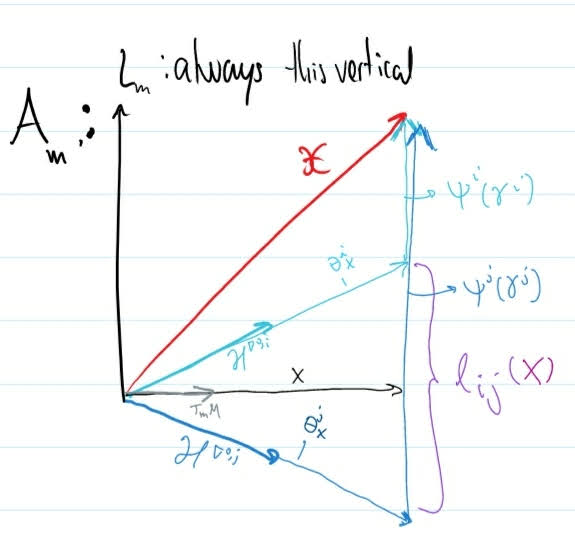
\includegraphics[width = \textwidth/2]{images/DiagramaMapasLocalesAlgebroide.jpg}
    \caption{Representation of the local maps introduced to study a transitive Lie algebroid $A$. The whole space represents, roughly, the vector space $A_m$ for $m \in M$, and $\oid X$ such that $a(\oid X) = X$ is an arbitrary element in $A_m$. Understanding $j$ as an inclusion, the vertical axis represents the adjoint Lie algebroid fiber $L_m$. The horizontal axis represents the tangent space $T_m M$, but it is not part of $A_m$, since there is no canonical horizontal direction in $A_m$. The images of $\Theta^i$ and $\Theta^j$ give two distinct notions of horizontality in $A_m$.}
    \label{fig:localMaps}
\end{figure}

\begin{theorem}
$\chi^i_j: U_{ij} \to U_{ij} \times \alg g$ is a Maurer-Cartan form, i.e. it satisfies the Maurer-Cartan equation:
\begin{align*}
    d \chi^i_j(X, Y) + [\chi^i_j(X), \chi^i_j(Y)] = 0
\end{align*} for all $X, Y \in TU_{ij}$.
\end{theorem}

\begin{proof}
Add proof is this theorem is indeed left in the document. This reduces to the fact that the standard flat connection in $U_i \times \alg g$ is mapped through $\psi^i$ to the adjoint connection $\nabla^{\Theta^i}$ in $L_{U_i}$ induced by the flat connection $\Theta^i$ in $A_{U_i}$. 
\end{proof}

%%%%%%%%%%%%%%%%%%%%%%%%%%%%%%%%%%%%%%%%%%%%%%%%%%%%%%%%%%%%%%%%%%%%%%%%%%%%%%%%%%%%
%%%%%%%%%%%%%%%%%%%%%%%%%%%%%%%%%%%%%%%%%%%%%%%%%%%%%%%%%%%%%%%%%%%%%%%%%%%%%%%%%%%%
\subsection{Local Description of the Atiyah Lie algebroid}

$\psi_i(\eta^i)(p) = Ad_{g^{-1}}\eta^i(x)$.

$\Theta^i(X)_p = R_{g*, s_i(x)} s_{i*, x} X_x$

If $X \oplus \eta^i$ and $X \oplus \eta^j$ are local trivializations of $\oid X$, $\sectoid X$, then

\begin{align}
    \eta^i &= g_{ij} \eta^j g_{ij}^{-1} + g_{ij} dg^{-1}_{ij}(X) \\
    \alpha^i_j(\eta) &= g_{ij} \eta  g_{ij}^{-1} \\
     \chi^i_j(X) &= g_{ij} dg_{ij}^{-1}(X) 
\end{align}

%\section{Actions of Lie Algebroids?}
%%%%%%%%%%%%%%%%%%%%%%%%%%%%%%%%%%%%%%%%%%%%%%%%%%%%%%%%%%%%%%%%%%%%%%%%%%%%%%%%%%%%
%%%%%%%%%%%%%%%%%%%%%%%%%%%%%%%%%%%%%%%%%%%%%%%%%%%%%%%%%%%%%%%%%%%%%%%%%%%%%%%%%%%%
%%%%%%%%%%%%%%%%%%%%%%%%%%%%%%%%%%%%%%%%%%%%%%%%%%%%%%%%%%%%%%%%%%%%%%%%%%%%%%%%%%%%
%%%%%%%%%%%%%%%%%%%%%%%%%%%%%%%%%%%%%%%%%%%%%%%%%%%%%%%%%%%%%%%%%%%%%%%%%%%%%%%%%%%%


